\documentclass[11pt]{amsart}
\usepackage[margin=1in]{geometry}
\usepackage[T1]{fontenc}
\usepackage{amsmath,amssymb,amsthm,mathtools,mathrsfs}
\usepackage{microtype,graphicx,nicefrac}
\usepackage[dvipsnames]{xcolor}
\usepackage[square,authoryear]{natbib}
\usepackage[citecolor=PineGreen,colorlinks=true,linkcolor=RoyalBlue,urlcolor=BrickRed]{hyperref}
\hypersetup{pdftitle={Sandpile avalanches in two dimensions are finite},pdfauthor={Ahmed Bou-Rabee}}
\setlength{\emergencystretch}{2em}
\numberwithin{equation}{section}
\newtheorem{theorem}[equation]{Theorem}
\newtheorem{proposition}[equation]{Proposition}
\newtheorem{lemma}[equation]{Lemma}
\newcommand{\Z}{\mathbb Z}
\newcommand{\PP}{\mathbb P}
\newcommand{\EE}{\mathbb E}
\newcommand{\nf}{\nicefrac}
\newcommand{\cL}{\mathscr{L}}
\DeclareMathOperator{\diam}{diam}
\title[Sandpile avalanches in two dimensions]{Sandpile avalanches in two dimensions are finite}
\author{Ahmed Bou-Rabee}
\begin{document}
\raggedbottom
\begin{abstract}
In the abelian sandpile model on~$\Z^d$, a site with at least~$2d$ grains topples by sending one grain to each neighbor. In a box~$[-N,N]^d$ whose boundary absorbs grains, adding grains at random sites and toppling defines a Markov chain. Athreya and J\'arai (2004) constructed the stationary state on~$\Z^d$ as the limit of its stationary distributions as~$N\to\infty$. By a formula of Dhar (1990), when a grain is added at the origin of a sandpile in the stationary state, the expected number of topplings at a site in the resulting avalanche is proportional to the Green function of simple random walk from the origin. This Green function is finite for~$d\geq3$, where J\'arai and Redig (2008) proved that avalanches are almost surely finite, and infinite for~$d=2$. We answer a question of Athreya and J\'arai (2004) by proving that for~$d=2$ avalanches are nevertheless almost surely finite: the probability that an avalanche reaches distance~$R$ is at most a negative power of~$\log R$.
\end{abstract}
\maketitle
\begin{figure}[!h]
\centering
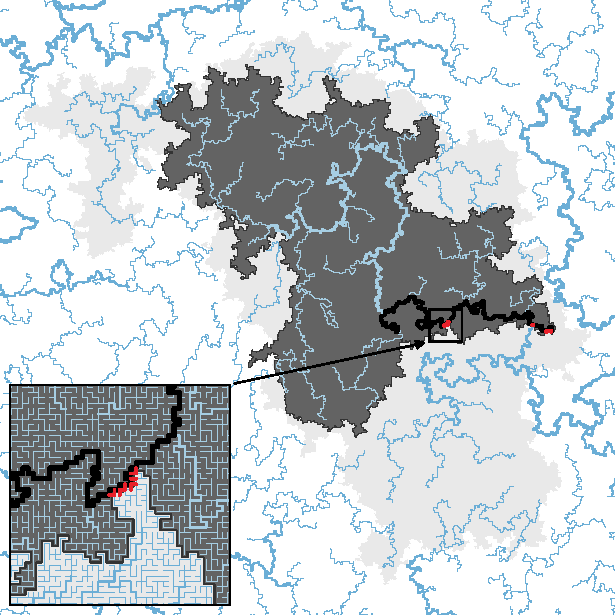
\includegraphics[width=0.63\textwidth]{figures/avalanche/figure.pdf}
\caption{An avalanche, in light gray, with one of its waves in dark gray. The burning bijection~\citep{MajumdarDhar1992}, applied separately to the wave and to the rest of the box, turns the sandpile left by the wave into two spanning trees, in light and darker blue. Joining them along a red edge makes the wave the set of vertices whose paths to the sink use that edge. The black paths join the origin, its neighbors, and a distant vertex.}
\label{fig:avalanche}
\end{figure}


\section{Introduction}\label{sec:introduction}

Consider a graph with a distinguished vertex called the \textbf{sink}. A \textbf{sandpile}~$\eta$ on the graph is a function from the set of non-sink vertices to the integers, where~$\eta(v)$ represents the number of grains, or \textbf{height}, at vertex~$v$. A sandpile~$\eta$ is \textbf{stable} if~$\eta(v)$ is less than the degree of~$v$ for every non-sink vertex~$v$. We call a vertex~$v$ \textbf{unstable} in~$\eta$ if~$v$ is not the sink and~$\eta(v)$ is at least the degree of~$v$. An unstable vertex~$v$ can \textbf{topple}, moving one grain along each edge from~$v$. Grains sent to the sink disappear. The topplings that follow the addition of a grain to a stable sandpile form an \textbf{avalanche} (Figure~\ref{fig:avalanche}). A box~$[-N,N]^d$ of~$\Z^d$ with \textbf{wired boundary conditions} is the graph obtained from~$\Z^d$ by identifying all vertices outside the box to a single vertex, the sink, and deleting the loops at the sink. On this graph every sandpile becomes stable after finitely many topplings, and adding grains at uniformly chosen vertices and toppling until the sandpile is stable defines a Markov chain on stable sandpiles.

\citet{Dhar1990} showed that, when a grain is added to a sandpile in the stationary distribution of this chain, the expected number of topplings at each vertex is proportional to the Green function of simple random walk in the box. As the box grows, this Green function stays bounded when~$d\geq3$ and grows logarithmically when~$d=2$~\citep{LawlerLimic2010}. \citet*{AthreyaJarai2004,AthreyaJarai2006} constructed the stationary state on~$\Z^d$ as the limit of these stationary distributions and asked whether avalanches are almost surely finite, expecting the transience or recurrence of random walk to play a role. \citet*{JaraiRedig2008} proved that the answer is yes when~$d\geq3$. When~$d=2$, \citet*{BhupatirajuHansonJarai2017} showed that the expected radius of an avalanche is infinite, but whether avalanches on~$\Z^2$ are almost surely finite has remained open~\citep*{JaraiRedig2008,JaraiWerning2014,Jarai2018}.


\subsection{Main result}\label{ssec:main-results}

In a box of~$\Z^2$ with wired boundary conditions, a stable sandpile~$\eta$ is \textbf{recurrent} if~$\eta$ can be obtained from every sandpile by a combination of adding grains and selectively toppling unstable vertices. The stationary distribution of the Markov chain above is uniform on recurrent sandpiles~\citep{Dhar1990}. Let~$\mu$ be the \textbf{stationary state} on~$\Z^2$, the local limit of these uniform measures as the box grows~\citep*{AthreyaJarai2004,AthreyaJarai2006}. The measure~$\mu$ is translation invariant.

For a sandpile~$\eta$, let~$\eta+\delta_0$ be the sandpile obtained by adding one grain at the origin. A toppling at~$v$ is \textbf{legal} if~$v$ is unstable in the current sandpile when the toppling occurs. If a finite sequence of topplings takes~$\eta+\delta_0$ to a stable sandpile, then~$\eta+\delta_0$ \textbf{stabilizes}. By the abelian property~\citep{Dhar1990}, the number~$u(x)$ of topplings at~$x$ does not depend on the sequence. We call~$u$ the \textbf{odometer} of the stabilization. The \textbf{radius} of the avalanche is~$\rho\coloneqq\max\{|x|_\infty:u(x)>0\}$, with~$\rho=0$ when no vertex topples and~$\rho=\infty$ when~$\eta+\delta_0$ does not stabilize.

\begin{theorem}\label{th:main}
For $\mu$-almost every sandpile~$\eta$, the sandpile~$\eta+\delta_0$ stabilizes. Moreover, there are constants~$a>0$ and~$C<\infty$ such that every~$M\geq0$ satisfies
\begin{equation*}
\mu(\rho>M)\leq C(\log(M+2))^{-a}\,.
\end{equation*}
\end{theorem}

Theorem~\ref{th:main} shows that avalanches on~$\Z^2$ are almost surely finite and so answers the question of~\citet*{AthreyaJarai2004} for~$d=2$.

\subsection{Proof overview}\label{ssec:proof-overview}

The main difficulty on~$\Z^2$ is that the origin topples infinitely many times in expectation~\citep*{BhupatirajuHansonJarai2017}. Physicists studied avalanches by splitting them into \textbf{waves}~\citep*{IvashkevichKtitarevPriezzhev1994}. While the origin is unstable, topple the origin once and then stabilize the other vertices, treating the origin as a sink; the vertices that topple form a wave. These topplings are legal, so when~$\eta+\delta_0$ stabilizes there are exactly~$u(0)$ waves, each finite, and each vertex topples at most once in each wave~\citep*{BhupatirajuHansonJarai2017}. Unlike an avalanche, a wave has an exact description. In a box, the sandpiles that waves leave behind in the stationary state correspond bijectively to two-component spanning forests, with the origin and the sink in different components, and the wave is the component of the origin~\citep{IvashkevichKtitarevPriezzhev1994}. \citet*{PriezzhevKtitarevIvashkevich1996} used this description, treating successive waves as nested, to predict the critical exponents of avalanches on~$\Z^2$.

Parts of this picture were made rigorous by~\citet*{BhupatirajuHansonJarai2017}. Summing over these forests counts each avalanche once for each of its waves, so their bound on the radius multiplies the probability that a single wave reaches a given distance by the expected number of waves. In boxes of~$\Z^2$ the expected number of waves grows like the logarithm of the size of the box, so this bound does not show that avalanches are finite.

Our proof takes waves as its starting point. We count only the waves that a large avalanche must contain, and we bound their number by an expectation over a uniform spanning tree of the box instead of a sum over two-component forests. The proof proceeds in three steps.
\begin{enumerate}
\item Fix integers~$r\geq2$ and~$M\geq r+2$, and mark the origin, its four neighbors, and the vertex~$(r,0)$. The origin is stable after the last wave, so the last wave misses a neighbor of the origin~\citep{BhupatirajuHansonJarai2017}. Hence an avalanche of radius larger than~$M$ has either a wave that misses a marked vertex and is not contained in the box of radius~$M$, or a wave that contains every marked vertex immediately followed by a wave that misses a marked vertex. We count only these waves and these pairs, and we bound their expected numbers by expectations over a uniform spanning tree of the box. The expected number of these pairs is at most~$\EE[\nf1\cL]$, where~$\cL$ is the number of lattice edges that join the tree paths between the marked vertices to vertices whose own paths to the sink avoid these tree paths. Step~1 below makes this definition precise.
\item At a single scale~$s$ reached by the tree paths between the marked vertices, the count~$\cL$ is at least~$\tfrac18\log s$ with probability at least a universal~$\varepsilon>0$, uniformly over the part of the tree on which we condition. In a finite domain that we compare with the lattice, the expected number of counted edges is an effective conductance, and most of the work goes into a bound on the variance of this number.
\item One scale gives only~$\EE[\nf1\cL]\leq1-\varepsilon+o(1)$, a bound that does not tend to zero as~$r$ grows. We construct the tree scale by scale, at scales whose logarithms grow geometrically, and apply Step~2 at each scale given the earlier ones. The conditional probabilities that the bound of Step~2 fails multiply, although the scales are not independent, and this gives~$\EE[\nf1\cL]\leq C(\log r)^{-a}$.
\end{enumerate}
\medskip

\noindent\textbf{Step 1.} The \textbf{uniform spanning tree} of a box with wired boundary conditions is a uniformly chosen spanning tree of the box, oriented toward the sink. The paths from the marked vertices to the sink eventually coincide. Their first common vertex~$v$ is the \textbf{common ancestor} of the marked vertices, and their segments up to and including~$v$ form the \textbf{minimal subtree} containing the marked vertices. The \textbf{past} of~$v$ is the set of vertices whose paths to the sink pass through~$v$. When~$v$ is not the sink, let~$\cL$ be the number of lattice edges, in the tree or not, with one endpoint in the minimal subtree and the other outside the past of~$v$. The first edge of the path from~$v$ to the sink is one of these edges, so~$\cL\geq1$. When~$v$ is the sink, let~$\cL\coloneqq\infty$.

In Proposition~\ref{sp:reciprocal-reduction}, we show that the radius of the avalanche exceeds~$M$ with probability at most the limit superior of~$\EE[\nf1\cL]$ as the box grows, plus~$Cr(M-r)^{-\nf13}$. The first term bounds the expected number of pairs of consecutive waves in which the first contains every marked vertex and the second does not. The second term bounds the expected number of waves that miss a marked vertex and are not contained in the box of radius~$M$. Such a wave has a boundary edge among the~$r+3$ lattice edges at the origin and on the segment from the origin to~$(r,0)$. In Lemma~\ref{rd:past-tail} we bound the probability that the past of a vertex in the uniform spanning tree of~$\Z^2$ is not contained in a large box around the vertex, using planar duality and a bound of~\citet*{BarlowMasson2011} on paths in the tree. The minimal subtree contains the origin and~$(r,0)$, so its diameter is at least~$r$, and Steps~2 and~3 use this to show that~$\cL$ is unlikely to be small. The proof of Theorem~\ref{th:main} takes~$r=\lfloor M^{\nf16}\rfloor$.

The first term comes from the following argument. Each recurrent sandpile of the box with the origin as an additional sink comes just before exactly one wave of exactly one avalanche from a recurrent sandpile, so a count over these sandpiles is a count over all waves of these avalanches. Fix a wave that contains every marked vertex. Adapting~\citet*{JaraiWerning2014}, we bound the number of sandpiles left by such waves by the number of pairs of recurrent sandpiles of the wave, with the origin as sink, and of the rest of the box. Start the next wave at the origin, and carry out legal topplings only at vertices whose four neighbors all lie in the wave that contains every marked vertex. These topplings form an initial part of the next wave. An argument of~\citet*{JaraiWerning2014} describes these topplings. For a uniformly chosen recurrent sandpile on the wave, the vertices that topple in this way have the law of the vertices whose paths to the origin, in a uniform spanning tree of the wave, avoid every vertex with a neighbor outside the wave. Hence the probability that the next wave misses a marked vertex is at most the probability that, in this tree, some lattice edge has one endpoint on the paths from the marked vertices to the origin and the other outside the wave. The new ingredient is to join this tree to a spanning tree of the complement of the wave along any one of these edges. The result is a spanning tree of the box, oriented toward the sink, in which the wave is the past of the common ancestor of the marked vertices and~$\cL$ is the number of these edges (Figures~\ref{fig:avalanche} and~\ref{fig:joining}). Each pair of trees with at least one such edge therefore produces~$\cL$ spanning trees of the box, all with the same value of~$\cL$, and weighting each of them by~$\nf1\cL$ counts the pair once. This bounds the expected number of such pairs of waves by~$\EE[\nf1\cL]$ for the uniform spanning tree of the box.

\begin{figure}[!ht]
\centering
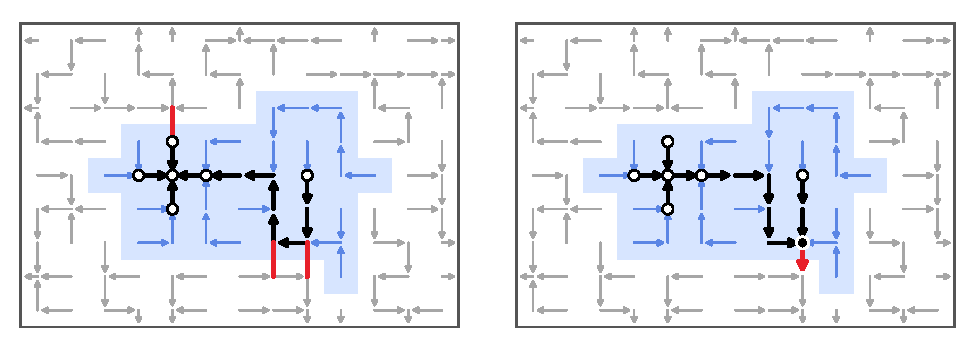
\includegraphics[width=\textwidth]{figures/joining/figure.pdf}
\caption{Left: a wave, shaded. The sandpile left by the wave gives a spanning tree of the wave oriented toward the origin, in blue, and a spanning tree of the rest of the box oriented toward the sink, in gray. The white discs are the origin, its four neighbors, and the vertex~$(4,0)$, which are the marked vertices. The black edges form the minimal subtree containing them, and the~$\cL=3$ red edges join this subtree to the rest of the box. Right: joining the two trees along one red edge reverses the orientation of the path from the endpoint of this edge in the wave to the origin. In the resulting spanning tree of the box, the black disc is the common ancestor of the marked vertices and the wave is the past of the black disc. Each red edge gives such a tree, so weighting each tree by~$\nf1\cL$ counts the pair of trees once.}
\label{fig:joining}
\end{figure}

\noindent\textbf{Step 2.} Since~$\nf1\cL\leq1$, we have~$\EE[\nf1\cL]\leq\PP(\cL<t)+\nf1t$ for every~$t>0$. A large mean of~$\cL$ does not bound~$\PP(\cL<t)$, since~$\cL$ could be large on a rare event and equal to one otherwise, so we bound~$\PP(\cL<t)$ directly. Suppose that~$v$ is not the sink, since otherwise~$\nf1\cL=0$, and call the path from~$v$ to the sink without~$v$ the path beyond~$v$. By Lemma~\ref{rd:conditional-law}, conditionally on the minimal subtree and the path beyond~$v$, the count~$\cL$ has the law of the count produced by Wilson's algorithm~\citep{Wilson1996} with these roots. From each remaining vertex in turn, a simple random walk runs until the walk hits a root or an earlier branch, and the loop erasure of the walk becomes a new branch. The path from a vertex along the branches ends at a root, and the vertex lies outside the past of~$v$ exactly when this root is on the path beyond~$v$, and~$\cL$ counts the edges from the minimal subtree to such vertices. In Proposition~\ref{fo:local-comparison}, we show that there is a universal~$\varepsilon>0$ such that, for every large integer~$s$ for which the minimal subtree reaches distance~$2s$ from~$v$, the probability that at least~$\tfrac18\log s$ of these edges start within distance~$2s$ of~$v$ is at least~$\varepsilon$.

To prove this, we replace the lattice by a finite domain, which Figure~\ref{fig:finite-domain} shows in the notation of Section~\ref{fo:section}. We add every vertex at distance at least~$2s$ from~$v$ to the minimal subtree as a root, and of the roots on the path beyond~$v$ we keep only a lattice path through them up to its first vertex at distance~$s$ from~$v$. A stochastic comparison of rooted spanning forests, which follows from~\citet{LyonsPeres2016}, shows that these changes stochastically shrink the set of vertices whose paths end on the path beyond~$v$. View the lattice as an electrical network of unit resistors. In the finite domain, the expected number of edges from the enlarged minimal subtree to vertices whose paths end on this lattice path equals the effective conductance between these two root sets. The~$s$ square circuits around~$v$ make this conductance at least~$\tfrac12\sum_{j=1}^s\nf1j$. In expectation, at most a constant number of these edges start at the added roots. The main technical difficulty is to bound the variance of the count uniformly over the shape of the domain, since this shape depends on the conditioning. The signed grove identities of~\citet*{KenyonWilson2009} give the probability that the count includes two given edges. In Section~\ref{sec:electrical} we sum this probability over pairs of edges and bound the variance, and in this domain the bound is at most a constant times the square of the mean. The proof uses the electrical square tiling of~\citet*{BrooksSmithStoneTutte1940}, which represents each edge with nonzero current by a square whose side is the current through the edge, so that these squares tile a rectangle (Figure~\ref{fig:electrical-tiling}). The Paley--Zygmund inequality then gives~$\varepsilon$.

\medskip
\noindent\textbf{Step 3.} We apply Step~2 at scales~$r_1<r_2<\cdots$, each a large fixed power of the previous one, and build the tree scale by scale. At scale~$r_i$, Wilson's algorithm starts walks from the vertices within distance~$3r_i+1$ of~$v$, which determines every edge counted by~$\cL$ that starts within distance~$3r_i$ of~$v$. Given the earlier scales, the rest of the construction is again Wilson's algorithm with the earlier branches as additional roots, so Step~2 applies at the next scale. One complication is that some of the edges that Step~2 finds may start on branches whose paths end on the minimal subtree, and~$\cL$ does not count these edges.

Two facts control these branches. By the discrete Beurling estimate of~\citet{Kesten1987}, a random walk rarely travels far without hitting the minimal subtree, so the branches added at scale~$r_i$ stay within distance~$r_i^6$ of~$v$, except with probability at most~$Cr_i^{-\nf12}$. Inside this box, in expectation at most a constant times~$\log r_i$ of the edges found at the next scale start on these branches, by an effective-conductance bound for the box joined to the path beyond~$v$ (Lemma~\ref{ct:needle} and Figure~\ref{fig:recentering}). Since~$r_{i+1}$ is a large power of~$r_i$, these edges are few compared with~$\log r_{i+1}$, and Lemma~\ref{ct:revealed-roots} shows that, with conditional probability at least~$\varepsilon/2$, at least~$\tfrac1{16}\log r_{i+1}$ edges start on the minimal subtree. The conditional failure probabilities, each at most~$1-\varepsilon/2$, multiply over the order~$\log\log r$ scales, up to the small probability that some branches leave their box, and this gives~$\EE[\nf1\cL]\leq C(\log r)^{-a}$.

\subsection{Related work}\label{ssec:related-work}

\subsubsection{Physics literature}
\citet*{BakTangWiesenfeld1987} introduced the abelian sandpile model as an example of self-organized criticality: in their simulations, avalanche sizes followed a power law, as at the critical point of a phase transition, but without the tuning of a parameter such as the temperature. Physicists predicted the exponents of these power laws on~$\Z^2$ by studying the waves of Section~\ref{ssec:proof-overview} and their two-component spanning forests~\citep{IvashkevichKtitarevPriezzhev1994}. \citet*{PriezzhevKtitarevIvashkevich1996} assumed that successive waves are nested with decreasing sizes and used scaling arguments to predict that exactly~$t$ vertices topple in an avalanche with probability of order~$t^{-\nf54}$. If the number of toppled vertices is of order the square of the radius, this prediction says that the radius of an avalanche exceeds~$R$ with probability of order~$R^{-\nf12}$, which is much smaller than the bound of Theorem~\ref{th:main}. Successive waves, however, need not be nested~\citep{DharManna1994}. \citet*{PaczuskiBoettcher1997} described how each wave repeats the topplings of the preceding wave up to the boundary of the preceding wave and can expand beyond that boundary, and~\citet*{KtitarevPriezzhev1998} observed that even a smaller wave need not lie inside its predecessor. \citet*{KtitarevLubeckGrassbergerPriezzhev2000} developed scaling predictions for waves from their two-component spanning forests, and~\citet*{DeMenechStella2000} found correlations between the sizes of successive waves. \citet*{TebaldiDeMenechStella1999} found numerical evidence that, unlike the number of toppled vertices, the number of topplings is not described by a single exponent. \citet*{JaraiSun2019} and~\citet{Sun2022} studied toppling probabilities and the number of waves numerically. Numerical work also suggests that the frontiers of avalanches~\citep*{Saberi2009} and the boundaries of waves~\citep*{AzimiTafreshi2010,DashtiNaserabadi2012} are described by the Schramm--Loewner evolution with parameter~$2$, the scaling limit of loop-erased random walk~\citep*{LawlerSchrammWerner2004}. Our proof does not assume that waves are nested.

\subsubsection{Infinite-volume sandpiles}
The burning bijection of~\citet*{MajumdarDhar1992} is a bijection between the recurrent sandpiles and the spanning trees of a finite graph, so the uniform measure on the recurrent sandpiles of a box is the image of the uniform spanning tree of the box. \citet*{AthreyaJarai2004,AthreyaJarai2006} constructed~$\mu$ by combining this bijection with the uniform spanning forest of~$\Z^d$, the limit of these trees, whose components are one-ended~\citep{Pemantle1991,BLPS2001}. Our proof uses the burning bijection separately on a wave and on the rest of the box. \citet{Jarai2012TransitiveGraphs} used a coupling to construct the stationary state on infinite graphs whose wired uniform spanning forest is connected and one-ended, and~\citet{JaraiWerning2014} removed the connectedness assumption when every component is one-ended. \citet*{GamlinJarai2014} constructed anchored burning bijections on such graphs, and on~$\Z^d$ they proved a power-law bound on the rate of convergence to the stationary state.

\subsubsection{Rigorous bounds on avalanches}
\citet*{BhupatirajuHansonJarai2017} showed that the last wave of an avalanche in a box is distributed as the component of the origin in a uniformly chosen two-component spanning forest, conditioned on a neighbor of the origin lying in the component of the sink. They also proved inequalities for the critical exponents of avalanches on~$\Z^d$ and bounded the radius of avalanches with a bounded number of waves. On~$\Z^2$, they showed that the~$k$th wave from the end, conditionally on its existence, converges in distribution to an almost surely finite set as the box grows. These results do not exclude infinitely many waves. For~$d\geq5$, \citet{Hutchcroft2020} determined the critical exponents of the radius and of the total number of topplings, and~\citet*{LiLiuShiraishi2026} announced these exponents for~$d=3$. On supercritical Galton--Watson trees conditioned to survive, \citet*{JaraiRuszelSaada2020} showed that an avalanche has more than~$t$ topplings with probability at most of order~$t^{-\nf12}$, and at least of this order when the offspring law has an exponential moment.

\subsection{Notation and conventions}

\begin{itemize}
\item We write~$|\cdot|_\infty$ for the maximum norm on the plane and~$\diam_\infty$ for the diameter in this norm.
\item For an integer~$r\geq0$, we also write~$[-r,r]^2$ for the set of points~$y\in\Z^2$ with~$|y|_\infty\leq r$, and we let~$\partial[-r,r]^2\coloneqq\{y\in\Z^2:|y|_\infty=r\}$. For~$x\in\Z^2$, we write~$x+[-r,r]^2$ and~$x+\partial[-r,r]^2$ for the translates of these sets by~$x$.
\item For a vertex~$x$ and a set~$V$ of vertices, let~$\deg(x,V)$ be the number of edges from~$x$ to~$V$.
\item We write~$\PP_y$ for the law of simple random walk from a vertex~$y$ on~$\Z^2$ or on a finite network, and the position at time zero counts as a visit.
\item When we identify vertices, as in wired boundary conditions, we delete loops, keep parallel edges, and count edges with multiplicity.
\item A sequence of laws of sandpiles or of spanning trees converges \textbf{locally} to a law when the probability of every event that depends only on finitely many heights or edges converges to the probability of this event under the limit law.
\item The value of~$C$ may change from one occurrence to the next.
\item We write~$\log$ for the natural logarithm.
\end{itemize}

\subsection{Formalization}\label{ssec:formalization}

A Lean~4 formalization accompanying this paper is maintained at
\begin{center}
\url{https://github.com/nitromannitol/finite-avalanche}
\end{center}
The development uses Mathlib together with explicitly listed standard results from the literature. The repository records the exact statements and sources of these inputs, the correspondence between the paper and the Lean declarations, and the current proof status.

\subsection*{Use of artificial intelligence}

The results of this paper were developed in collaboration with GPT-5.5 and models from the GPT-6 family from late May through early October 2026. The author directed the investigation, and the models contributed mathematical ideas, proof attempts, computations, counterexamples, and revisions. Claude Opus~5.5 made the figures and helped with the exposition.

We began by looking for exact maps between the waves of an avalanche, hoping to describe the complete avalanche through the two-component spanning forests of single waves. With the models, we enumerated all sandpiles in small boxes to test the proposed maps, including maps between the first and last waves. These computations ruled out every proposed identification of the complete avalanche with a single forest component: successive waves need not be nested, and the proposed maps did not preserve the uniform measure.

We then looked for a way to count complete avalanches instead of single waves. The models proposed candidate bijections and tested them by exact enumeration, and this search led to a bound on the probability of a large avalanche by a quantity defined through the uniform spanning tree, in which the number of waves no longer appears.

We then had to show that this quantity tends to zero. The models proposed proof routes and found counterexamples to several of them: estimates of means were not enough, and we needed a probability bound that survives revealing part of the tree. We first used such a bound to prove that avalanches are finite, and then applied the bound at many scales to obtain the logarithmic tail bound.

Throughout the investigation, separate agents pursued competing ideas and checked proposed proofs. We recorded each failed approach with the reason for its failure, so that later attempts did not repeat the approach. The author takes responsibility for the mathematical content and presentation of the paper.

\subsection*{Acknowledgments}

The author thanks Tom Hutchcroft, Xinyi Li, Antal J\'arai, Christoforos Panagiotis, and Runsheng Liu for useful conversations.

\section{Preliminaries}\label{sec:prelim}

\subsection{Spanning trees}\label{ssec:prelim-trees}

For a finite multigraph~$G$, let~$\tau(G)$ be the number of spanning trees of~$G$, with~$\tau(G)=1$ when~$G$ is a single vertex and~$\tau(G)=0$ when~$G$ is disconnected. Given a set of vertices of~$G$ called roots, a \textbf{rooted spanning forest} of~$G$ is an acyclic spanning subgraph in which every component contains exactly one root, and we use the same definition on~$\Z^2$ when the set of roots has finite complement. Identifying the roots to a single vertex turns the rooted spanning forests of~$G$ or of~$\Z^2$ into the spanning trees of the resulting finite multigraph. When the roots have colors, each vertex of a rooted spanning forest receives the color of the root of its component.

For an integer~$N\geq1$, we also write~$[-N,N]^2$ for the box~$[-N,N]^2$ with wired boundary conditions, and~$s_N$ for its sink. Let~$T_N$ be a uniform spanning tree of~$[-N,N]^2$, oriented toward~$s_N$. The law of~$T_N$ converges locally as~$N\to\infty$ to the law of the \textbf{uniform spanning tree}~$T$ of~$\Z^2$, and~$T$ is almost surely a spanning tree of~$\Z^2$ with one end~\citep[Theorems~6.1 and~6.3(i)]{Jarai2018}. Orient~$T$ toward its end.

Let~$t$ be either~$T$ or a finite tree oriented toward a root. Every vertex of~$t$ other than the root has exactly one outgoing edge, and the \textbf{oriented path} from a vertex~$x$ of~$t$ starts at~$x$ and follows the outgoing edges. In~$T$ this path is infinite. The \textbf{past}~$\operatorname{Past}_t(x)$ of a vertex~$x$ is the set of vertices whose oriented paths pass through~$x$. Every past in~$T$ is finite because~$T$ has one end. For a finite nonempty set of vertices of~$t$, the oriented paths from these vertices eventually coincide, and their first common vertex is the \textbf{common ancestor} of the set.

Fix a finite nonempty set~$S\subset\Z^2$, which from Section~\ref{rd:section} on is the set defined there. When~$t$ is a tree in~$[-N,N]^2$ that contains~$S$, the segments of the oriented paths from the vertices of~$S$ up to their common ancestor form the \textbf{minimal subtree}~$K_t$ of~$t$ containing~$S$, and~$K_t$ also denotes the vertex set of this subtree. The set~$K_t$ contains the common ancestor of~$S$ and lies in the past of the common ancestor. When the common ancestor of~$S$ is not~$s_N$, let~$\cL_t$ be the number of lattice edges, in~$t$ or not, from~$K_t$ to vertices outside the past of the common ancestor of~$S$. When the common ancestor of~$S$ is~$s_N$, let~$\cL_t\coloneqq\infty$, so that~$\cL_t^{-1}=0$. An edge to~$s_N$ is a lattice edge from~$[-N,N]^2$ to~$\Z^2\setminus[-N,N]^2$. Hence, unless the common ancestor of~$S$ is the root of~$t$, the outgoing edge of the common ancestor is one of the edges counted by~$\cL_t$, and~$\cL_t\geq1$. The common ancestor and its past appear in~\citet[Section~3.1]{AthreyaJarai2004}, and~$K_t$ is the set called the span in~\citet[page~2 of the electronic supplement]{AthreyaJarai2006}.

For a vertex~$x$ and a finite set of vertices, the past of~$x$ in~$T$, and in~$T_N$ when~$[-N,N]^2$ contains the set, equals the set exactly when the edges of the tree with an endpoint in the set form a spanning tree of the set together with one edge from~$x$ to a vertex outside the set~\citep[proof of Claim~1 of the electronic supplement]{AthreyaJarai2006}. Hence, for every integer~$M\geq0$, the event that the past of~$x$ lies in~$[-M,M]^2$ depends only on the edges with an endpoint in~$[-M,M]^2$, in~$T$ and in~$T_N$ when~$N\geq M$, and the local convergence of~$T_N$ to~$T$ gives
\begin{equation}\label{pre:past-limit}
\PP\bigl(\operatorname{Past}_{T_N}(x)\subset [-M,M]^2\bigr)\to\PP\bigl(\operatorname{Past}_T(x)\subset [-M,M]^2\bigr)\quad\text{as }N\to\infty\,.
\end{equation}

\subsection{Sandpiles}\label{ssec:prelim-sandpiles}

Let~$G$ be a finite connected loopless multigraph with a sink, and define recurrent sandpiles on~$G$ as in Section~\ref{ssec:main-results}. A nonempty set of non-sink vertices is a \textbf{forbidden subconfiguration} of a sandpile~$\eta$ when the height~$\eta(x)$ of every vertex~$x$ of the set is less than the number of edges from~$x$ to the set.

Let~$\eta$ be a stable sandpile on~$G$, and fix a set of non-sink vertices to hold unburned. \textbf{Burning}~$\eta$ from the sink while holding these vertices unburned proceeds in steps. The sink burns at step zero, and each later step burns every unburned vertex that is not held and whose height is at least the number of its edges to the vertices unburned at the start of the step. The procedure stops when a step burns no vertex, and the vertices that are still unburned form the final unburned set. With no held vertex, this procedure is the burning algorithm of~\citet[Section~4.1]{Jarai2018}, and in general the procedure is the first phase of the burning in~\citet[Section~3.1]{JaraiWerning2014}.

The following facts go back to~\citet{Dhar1990} and~\citet{MajumdarDhar1992}. By~\citet[Exercise~4.5]{Jarai2018}, every stable sandpile~$\eta$ on~$G$ satisfies
\begin{equation}\label{pre:burning}
\eta\text{ is recurrent}\quad\text{exactly when}\quad\eta\text{ has no forbidden subconfiguration}\,.
\end{equation}
By~\citet[Corollary~4.4]{Jarai2018}, the burning algorithm gives a bijection between the recurrent sandpiles on~$G$ and the spanning trees of~$G$, so
\begin{equation}\label{pre:count}
\bigl|\{\text{recurrent sandpiles on }G\}\bigr|=\tau(G)\,.
\end{equation}
By~\citet[Theorem~2.11 and Section~2.3]{Jarai2018},
\begin{equation}\label{pre:permutation}
\text{adding a grain at a non-sink vertex and stabilizing permutes the recurrent sandpiles on~$G$}\,.
\end{equation}

The next lemma restates an observation in~\citet[proof of Theorem~3]{JaraiWerning2014}; see also~\citet[Lemmas~3 and~4]{GamlinJarai2014}.

\begin{lemma}\label{fv:held-burning}
Let~$G$ be a finite connected loopless multigraph with a sink. Burn a uniform recurrent sandpile on~$G$ from the sink while holding a set of non-sink vertices unburned. Then the final unburned set has the law of the union of the pasts of the held vertices in a uniform spanning tree of~$G$ oriented toward the sink.
\end{lemma}

\begin{proof}
Continue the burning in steps in a second phase without holding any vertex. The two phases together define a bijection between the recurrent sandpiles on~$G$ and the spanning trees of~$G$ oriented toward the sink~\citep[Section~3.1]{JaraiWerning2014}. In this bijection, the outgoing edge of a vertex that burns at the first step of the second phase leads to a vertex burned in the first phase, and the outgoing edge of every other vertex leads to a vertex that burned at the previous step. Hence the oriented path from every vertex burned in the first phase avoids the held vertices. Every vertex of the final unburned set of the first phase that is not held has height less than the number of its edges to this set, so only held vertices burn at the first step of the second phase, and the oriented path from every vertex of this set meets a held vertex. Thus the final unburned set is the union of the pasts of the held vertices in the corresponding tree.
\end{proof}

Let~$\mu_N$ be the uniform measure on the recurrent sandpiles of~$[-N,N]^2$. By~\citet[Theorem~1]{AthreyaJarai2004}, with the correction in~\citet{AthreyaJarai2006},
\begin{equation}\label{pre:sandpile-limit}
\mu_N\to\mu\quad\text{locally as }N\to\infty\,.
\end{equation}

\subsection{Wilson's algorithm with two root sets}\label{ssec:prelim-wilson}

Fix a nonempty set of roots in a finite connected multigraph, or a set of roots in~$\Z^2$ with finite complement, and fix an enumeration of the vertices. \textbf{Wilson's algorithm}~\citep{Wilson1996} visits the vertices in the order of the enumeration. From each visited vertex that is neither a root nor on an earlier \textbf{branch}, an independent simple random walk runs until the walk hits a root or an earlier branch, and the chronological loop erasure of the walk becomes a new branch. Wilson's theorem~\citep[Theorem~4.1]{LyonsPeres2016}, applied to the finite connected multigraph obtained by identifying the roots to a single vertex, shows that for every enumeration
\begin{equation}\label{pre:wilson}
\text{the branches form the uniform rooted spanning forest with the given roots}\,.
\end{equation}

Let~$A$ and~$\Gamma$ be disjoint nonempty sets of vertices, and run Wilson's algorithm with roots~$A\cup\Gamma$, where the vertices of~$A$ are the roots of color zero and the vertices of~$\Gamma$ are the roots of color one. When~$A$ and~$\Gamma$ are subsets of~$\Z^2$ whose union has finite complement, let~$\nu_{A,\Gamma}$ be the law of the colors of the forest formed by the branches. By~\eqref{pre:wilson}, this law does not depend on the enumeration. Enumerating a vertex~$y$ first gives
\begin{equation}\label{fo:color-marginal}
\nu_{A,\Gamma}(\text{$y$ has color one})=\PP_y(\text{the walk visits~$\Gamma$ before~$A$})\,.
\end{equation}
For a set~$V\subset\Z^2$, let~$\cL(V)$ be the number of lattice edges from~$V$ to vertices of color one.

\begin{lemma}\label{fo:lattice-monotonicity}
Let~$A\subset A'$ and~$\Gamma'\subset\Gamma$ be subsets of~$\Z^2$ for which~$\nu_{A,\Gamma}$ and~$\nu_{A',\Gamma'}$ are defined. Then the set of vertices of color one under~$\nu_{A',\Gamma'}$ is stochastically smaller than under~$\nu_{A,\Gamma}$.
\end{lemma}

\begin{proof}
Starting from the roots~$A$ of color zero and~$\Gamma$ of color one, we remove the roots in~$\Gamma\setminus(A'\cup\Gamma')$, which leaves the roots~$(A\cup\Gamma)\cap(A'\cup\Gamma')$, and then make every vertex of~$A'\setminus A$ a root of color zero, which gives the roots~$A'$ of color zero and~$\Gamma'$ of color one. Every set of roots in these steps has finite complement, since~$A\cup\Gamma$ and~$A'\cup\Gamma'$ do. Identifying the roots turns the rooted spanning forests of~$\Z^2$ into the spanning trees of the resulting finite multigraphs, and enlarging the set of roots identifies further vertices. By~\citet[Exercise~10.8 and Theorem~10.4]{LyonsPeres2016}, there is therefore a coupling in which the forest with more roots is contained in the forest with fewer roots. Removing roots of color one keeps each old component of color zero inside the new component of its root. Making vertices roots of color zero splits each old component of color zero into components of color zero. In both steps every vertex of color zero keeps its color.
\end{proof}

\subsection{Electrical networks and random walk}\label{ssec:prelim-electrical}

We view a multigraph as an electrical network in which every edge has conductance one, and a sum over~$xy$ has one term for each edge, with parallel edges counted separately. The \textbf{energy} of a function~$f$ on the vertices is~$\sum_{xy}(f(x)-f(y))^2$. Let~$A$ and~$\Gamma$ be disjoint nonempty sets of vertices of a finite connected network. The \textbf{voltage} between~$A$ and~$\Gamma$ is the function that equals one on~$A$ and zero on~$\Gamma$ and is harmonic at every other vertex. The \textbf{current} of the voltage through an edge from~$x$ to~$y$ is the voltage at~$x$ minus the voltage at~$y$, and the \textbf{effective conductance} between~$A$ and~$\Gamma$ is the energy of the voltage and is symmetric in~$A$ and~$\Gamma$. The reciprocal of the effective conductance is the \textbf{effective resistance}. By~\citet[equation~(2.2) and the uniqueness principle in Section~2.1]{LyonsPeres2016}, every vertex~$y$ satisfies
\begin{equation}\label{pre:voltage}
\text{the voltage between~$A$ and~$\Gamma$ at~$y$}=\PP_y(\text{the walk visits~$A$ before~$\Gamma$})\,.
\end{equation}
By Dirichlet's principle~\citep[Exercises~2.13 and~2.79]{LyonsPeres2016},
\begin{equation}\label{pre:dirichlet}
\text{the effective conductance between~$A$ and~$\Gamma$}=\min_f\sum_{xy}(f(x)-f(y))^2\,,
\end{equation}
where~$f$ runs over the functions that equal one on~$A$ and zero on~$\Gamma$. By~\citet[Exercise~2.47 and equation~(2.7)]{LyonsPeres2016},
\begin{equation}\label{pre:count-conductance}
\sum_{xy:\,x\in A}\PP_y(\text{the walk visits~$\Gamma$ before~$A$})=\text{the effective conductance between~$A$ and~$\Gamma$}\,.
\end{equation}

Let~$A$ and~$\Gamma$ be disjoint nonempty subsets of~$\Z^2$ such that one of them is finite and the other has finite complement. We take the voltage and the effective conductance between~$A$ and~$\Gamma$ in the finite network obtained from~$\Z^2$ by identifying~$A$ to one vertex and~$\Gamma$ to another, and we view the voltage and the functions in~\eqref{pre:dirichlet} as functions on~$\Z^2$.

Let~$r\geq1$ be an integer. For~$r\leq j\leq2r-1$, the~$8j+4$ edges from~$\partial[-j,j]^2$ to~$\partial[-j-1,j+1]^2$ separate~$[-r,r]^2$ from~$\Z^2\setminus [-2r+1,2r-1]^2$, and these~$r$ sets of edges are disjoint. The Nash-Williams inequality~\citep[Section~2.5]{LyonsPeres2016} therefore bounds the effective resistance between~$[-r,r]^2$ and~$\Z^2\setminus [-2r+1,2r-1]^2$ below by~$\sum_{j=r}^{2r-1}(8j+4)^{-1}\geq\nf1{16}$, so
\begin{equation}\label{pre:annulus}
\text{the effective conductance between~$[-r,r]^2$ and~$\Z^2\setminus [-2r+1,2r-1]^2$ is at most~$16$}\,.
\end{equation}

Let~$r\geq2$ be an integer, and let~$K$ be a connected set of lattice vertices that contains~$0$ and meets~$\partial[-r^6,r^6]^2$. The open Euclidean disk of radius~$6r+4$ about~$0$ contains~$[-3r-1,3r+1]^2$, and the open Euclidean disk of radius~$r^6$ about~$0$ contains the first disk and misses~$\partial[-r^6,r^6]^2$. The discrete Beurling estimate of~\citet{Kesten1987}, in the form of~\citet[Lemma~2.1]{Lawler2020} for these two disks, applied to the initial segment of a simple path in~$K$ from~$0$ to~$\partial[-r^6,r^6]^2$ up to its first exit from the larger disk, gives
\begin{equation}\label{ct:beurling}
\sup_{x\in [-3r-1,3r+1]^2}\PP_x(\text{the walk visits~$\partial[-r^6,r^6]^2$ strictly before~$K$})\leq Cr^{-\nf52}\,.
\end{equation}

\section{Reduction to the uniform spanning tree}\label{rd:section}

In this section we deduce Theorem~\ref{th:main} from three results. Proposition~\ref{sp:reciprocal-reduction}, which we prove in Section~\ref{sp:section}, bounds the tail of the radius by the expected reciprocal of the count~$\cL$ for the uniform spanning tree of a large box, plus~$Cr(M-r)^{-\nf13}$. Lemma~\ref{rd:conditional-law}, which we prove here, shows that, when the common ancestor is not the sink, the conditional law of~$\cL$ given the minimal subtree and the path from the common ancestor to the sink is the law of a count of edges for Wilson's algorithm with two root sets. Proposition~\ref{ct:reciprocal}, which we prove in Sections~\ref{fo:section}--\ref{sec:electrical}, bounds the expected reciprocal of this count by a negative power of the logarithm of the diameter of the minimal subtree, uniformly over the root sets.

For an integer~$r\geq2$, let~$S$ be the set consisting of the origin, its four neighbors, and the vertex~$(r,0)$. Then~$\cL_{T_N}$ is the count~$\cL$ of Section~\ref{ssec:proof-overview} for the uniform spanning tree of~$[-N,N]^2$.

\begin{proposition}\label{sp:reciprocal-reduction}
There is a universal constant~$C<\infty$ such that all integers~$r\geq2$ and~$M\geq r+2$ satisfy
\begin{equation}\label{sp:reduction-bound}
\mu(\rho>M)\leq\limsup_{N\to\infty}\EE\bigl[\cL_{T_N}^{-1}\bigr]+Cr(M-r)^{-\nf13}\,.
\end{equation}
\end{proposition}

We bound~$\EE[\cL_{T_N}^{-1}]$ by conditioning on~$K_{T_N}$ and on the path in~$T_N$ from the common ancestor of~$S$ to~$s_N$.

\begin{lemma}\label{rd:conditional-law}
Let~$N\geq r$. On the event that the common ancestor of~$S$ in~$T_N$ is not~$s_N$, let~$\Gamma_N$ be the union of~$\Z^2\setminus [-N,N]^2$ and the set of vertices of~$[-N,N]^2$ that follow the common ancestor on the path in~$T_N$ from the common ancestor to~$s_N$. Then, on this event, the set~$\Gamma_N$ avoids~$K_{T_N}$, and the conditional law of~$\cL_{T_N}$ given~$K_{T_N}$ and this path is the law of~$\cL(K_{T_N})$ under~$\nu_{K_{T_N},\Gamma_N}$.
\end{lemma}

\begin{proof}
By~\eqref{pre:wilson}, Wilson's algorithm on~$[-N,N]^2$ with the single root~$s_N$ generates~$T_N$ for every enumeration, and we enumerate the vertices of~$S$ first. The branches from the vertices of~$S$ form~$K_{T_N}$ together with the path in~$T_N$ from the common ancestor of~$S$ to~$s_N$. Given these branches, the later walks use new independent increments and carry out Wilson's algorithm with the vertices of these branches as roots, where the vertices of~$K_{T_N}$ have color zero and the other vertices of these branches have color one. Suppose that the common ancestor is not~$s_N$. The vertices of~$\Gamma_N$ in~$[-N,N]^2$ follow the common ancestor on its path and therefore lie outside the past of the common ancestor, which contains~$K_{T_N}$, so~$\Gamma_N$ avoids~$K_{T_N}\subset [-N,N]^2$. Since a step out of~$[-N,N]^2$ is a step to~$s_N$ in~$[-N,N]^2$, Wilson's theorem~\eqref{pre:wilson} shows that the conditional law of the colors in~$[-N,N]^2$ given these branches is their law under~$\nu_{K_{T_N},\Gamma_N}$. This law depends only on~$K_{T_N}$ and on the path, so this law is also the conditional law of the colors given~$K_{T_N}$ and the path. A vertex has color zero exactly when the oriented path from the vertex passes through the common ancestor, so the vertices of color zero form the past of the common ancestor, and~$\cL_{T_N}$ is the number of edges of~$[-N,N]^2$ from~$K_{T_N}$ to vertices of color one. Hence the conditional law of~$\cL_{T_N}$ given~$K_{T_N}$ and the path is the law of~$\cL(K_{T_N})$ under~$\nu_{K_{T_N},\Gamma_N}$.
\end{proof}

Let~$K$ be a finite connected set of lattice vertices, and let~$\gamma\subset\Z^2\setminus K$ be a connected set with finite complement that contains a neighbor of a vertex of~$K$. Under~$\nu_{K,\gamma}$, some edge joins~$K$ to a vertex of~$\gamma$, which is a root of color one, so the count~$\cL(K)$ of Section~\ref{ssec:prelim-wilson} satisfies~$\cL(K)\geq1$.

\begin{proposition}\label{ct:reciprocal}
There are universal constants~$a>0$ and~$C<\infty$ such that every~$K$ and~$\gamma$ as above satisfy
\begin{equation*}
\EE_{\nu_{K,\gamma}}\bigl[\cL(K)^{-1}\bigr]\leq C\bigl(\log(\diam_\infty K+2)\bigr)^{-a}\,.
\end{equation*}
\end{proposition}

\begin{proof}[Proof of Theorem~\ref{th:main} assuming Propositions~\ref{sp:reciprocal-reduction} and~\ref{ct:reciprocal}]
Let~$N\geq r$, and suppose that the common ancestor of~$S$ in~$T_N$ is not~$s_N$. By Lemma~\ref{rd:conditional-law}, the set~$\Gamma_N$ avoids~$K_{T_N}$. The set~$\Gamma_N$ has finite complement and is connected, since~$\Z^2\setminus [-N,N]^2$ is connected and the path ends with an edge to~$s_N$. The lattice edge that corresponds to the outgoing edge of the common ancestor joins the common ancestor, which lies in~$K_{T_N}$, to a vertex of~$\Gamma_N$. Since~$K_{T_N}$ contains the origin and~$(r,0)$, the diameter of~$K_{T_N}$ is at least~$r$. Since also~$\cL_{T_N}^{-1}=0$ when the common ancestor is~$s_N$, Lemma~\ref{rd:conditional-law} and Proposition~\ref{ct:reciprocal} with~$K=K_{T_N}$ and~$\gamma=\Gamma_N$ give~$\EE[\cL_{T_N}^{-1}]\leq C(\log(r+2))^{-a}$ for every~$N\geq r$. For an integer~$M\geq64$, let~$r\coloneqq\lfloor M^{\nf16}\rfloor$, so that~$r\geq2$ and~$M\geq r+2$. Then~\eqref{sp:reduction-bound} gives
\begin{equation*}
\mu(\rho>M)\leq C(\log(r+2))^{-a}+Cr(M-r)^{-\nf13}\leq C(\log(M+2))^{-a}\,.
\end{equation*}
Increasing~$C$ extends this bound to all real~$M\geq0$, and letting~$M$ tend to infinity shows that~$\eta+\delta_0$ stabilizes for $\mu$-almost every~$\eta$.
\end{proof}


\section{From avalanches to spanning trees}\label{sp:section}

In this section we prove Proposition~\ref{sp:reciprocal-reduction}. Fix integers~$r\geq2$ and~$M\geq r+2$, and let~$S$ be as in Section~\ref{rd:section}. For a recurrent sandpile~$\eta$ on~$[-N,N]^2$, we also write~$\rho$ for the radius of the avalanche of~$\eta+\delta_0$ on~$[-N,N]^2$. Sections~\ref{ssec:waves} and~\ref{ssec:waves-to-trees} bound~$\mu_N(\rho>M)$ for a fixed integer~$N>M+1$, and Section~\ref{sec:limits} lets~$N\to\infty$.

\subsection{Waves}\label{ssec:waves}

Let~$X$ be the set of recurrent sandpiles on~$[-N,N]^2$ with~$0$ as an additional sink. For a sandpile~$\omega$ on~$[-N,N]^2\setminus\{0\}$, let~$\omega(0)\coloneqq-1$. By~\eqref{pre:burning}, the set~$X$ consists of the stable~$\omega$ with no forbidden subconfiguration avoiding~$0$. For~$\omega\in X$, let~$W(\omega)$ be the union of all forbidden subconfigurations of~$\omega$. A union of forbidden subconfigurations is a forbidden subconfiguration, and so is~$\{0\}$. Hence~$W(\omega)$ is the largest forbidden subconfiguration, and~$W(\omega)$ contains~$0$.

Let~$U$ act on~$X$ by adding one grain to each neighbor of~$0$ and stabilizing with both~$0$ and~$s_N$ as sinks. Since adding grains permutes recurrent sandpiles by~\eqref{pre:permutation}, the operator~$U$ is a permutation of~$X$. This operator appears in~\citet[equations~(7.1) and~(7.3)]{JaraiRedig2008}. To form the wave from~$\omega\in X$, give the origin height four, topple the origin once, and then stabilize the other vertices with~$0$ as a sink. The resulting sandpile away from the origin is~$U\omega$. The next lemma makes precise an observation of~\citet*[Section~2]{IvashkevichKtitarevPriezzhev1994}.

\begin{lemma}\label{fv:inverse-waves}
Let~$\omega\in X$. The wave from~$\omega$ topples exactly the vertices of~$W(U\omega)$, each once.
\end{lemma}

\begin{proof}
Each vertex other than the origin topples at most once in a wave~\citep*[Section~2.2]{BhupatirajuHansonJarai2017}. Let~$W$ be the set of vertices that topple in the wave from~$\omega$, including~$0$. On~$W\setminus\{0\}$ we have~$(U\omega)(x)=\omega(x)-4+\deg(x,W)<\deg(x,W)$. Hence~$W$ is a forbidden subconfiguration of~$U\omega$ with height~$-1$ at the origin, and~$W\subset W(U\omega)$. Every~$x\in W(U\omega)\setminus W$ satisfies
\begin{equation*}
 \omega(x)+\deg(x,W)=(U\omega)(x)<\deg\bigl(x,W(U\omega)\bigr)\leq\deg\bigl(x,W(U\omega)\setminus W\bigr)+\deg(x,W)\,,
\end{equation*}
so~$W(U\omega)\setminus W$ is empty, since otherwise this set would be a forbidden subconfiguration of~$\omega$ avoiding~$0$. Thus~$W=W(U\omega)$.
\end{proof}

By~\eqref{pre:burning}, the sandpiles that are recurrent on~$[-N,N]^2$ with an added edge from~$0$ to~$s_N$ but not recurrent on~$[-N,N]^2$ are the extensions of the sandpiles of~$X$ by height four at the origin. Hence, by~\citet[Definition~1 and Lemma~2.7]{BhupatirajuHansonJarai2017}, for every recurrent sandpile~$\eta$ on~$[-N,N]^2$ with~$\eta(0)=3$, the sandpile just before each wave of the avalanche of~$\eta+\delta_0$ is the extension of a sandpile of~$X$ by height four at the origin, and every sandpile of~$X$ is the sandpile away from the origin just before exactly one wave of exactly one of these avalanches. Each wave is the wave from the sandpile away from the origin just before this wave. By Lemma~\ref{fv:inverse-waves}, the wave from such a sandpile~$\omega$ topples exactly~$W(U\omega)$, and the preceding wave, if there is one, leaves~$\omega$ and therefore topples exactly~$W(\omega)$.

Let~$\eta$ be a recurrent sandpile on~$[-N,N]^2$ such that the avalanche of~$\eta+\delta_0$ has radius~$\rho>M$. Then~$\eta(0)=3$, since adding a grain at~$0$ to a recurrent sandpile with height at most two at the origin causes no toppling. The last wave misses a neighbor of~$0$~\citep[Corollary~2.8]{BhupatirajuHansonJarai2017} and therefore does not contain~$S$. Hence either some wave neither contains~$S$ nor lies in~$[-M,M]^2$, or a wave not containing~$S$ immediately follows a wave containing~$S$. The sandpile~$\omega$ away from the origin just before the wave in the first case satisfies~$S\not\subset W(U\omega)$ and~$W(U\omega)\not\subset [-M,M]^2$, and the sandpile~$\omega$ away from the origin just before the later wave in the second case satisfies~$S\subset W(\omega)$ and~$S\not\subset W(U\omega)$. By the previous paragraph, distinct sandpiles~$\eta$ give distinct sandpiles~$\omega$. Since~$\mu_N$ gives mass~$\tau([-N,N]^2)^{-1}$ to each recurrent sandpile by~\eqref{pre:count}, and since~$U$ is a permutation of~$X$, we obtain
\begin{equation}\label{fv:excursion-union}
\begin{split}
\mu_N(\rho>M)&\leq\tau([-N,N]^2)^{-1}\bigl|\{\omega\in X:S\subset W(\omega),\ S\not\subset W(U\omega)\}\bigr|\\
&\quad+\tau([-N,N]^2)^{-1}\bigl|\{\omega\in X:S\not\subset W(\omega),\ W(\omega)\not\subset [-M,M]^2\}\bigr|\,.
\end{split}
\end{equation}

\subsection{From waves to spanning trees}\label{ssec:waves-to-trees}

We bound the two terms of~\eqref{fv:excursion-union} by spanning-tree counts. Fix a set~$W$ with~$0\in W\subset [-N,N]^2$, and let~$W^c$ be the complement of~$W$ in the vertex set of the graph~$[-N,N]^2$, which contains~$s_N$. We also write~$W$ and~$W^c$ for the subgraphs of~$[-N,N]^2$ that these sets induce, with sinks~$0$ and~$s_N$. On each of these two graphs we count the stable sandpiles with no forbidden subconfiguration. By~\eqref{pre:burning}, these are the recurrent sandpiles when the graph is connected. When the graph is disconnected, there are none, since a component without the sink is a forbidden subconfiguration of every stable sandpile.

As in~\citet[proof of Theorem~3]{JaraiWerning2014}, restricting~$\omega$ to~$W\setminus\{0\}$ and taking~$\omega-\deg(\cdot,W)$ on~$[-N,N]^2\setminus W$ maps the sandpiles~$\omega\in X$ with~$W(\omega)=W$ injectively to pairs of such sandpiles on~$W$ and on~$W^c$. Indeed, suppose that~$W(\omega)=W$. The restriction of~$\omega$ to~$W\setminus\{0\}$ is stable because~$W$ is a forbidden subconfiguration, and a forbidden subconfiguration of this restriction would be one of~$\omega$ avoiding~$0$. Maximality of~$W$ makes~$\omega-\deg(\cdot,W)$ free of forbidden subconfigurations on~$[-N,N]^2\setminus W$, and~$\omega-\deg(\cdot,W)$ is stable because~$\omega\leq3$.

Counting the pairs with~\eqref{pre:count} gives
\begin{equation}\label{fv:shape-mass}
 \bigl|\{\omega\in X:W(\omega)=W\}\bigr|\leq\tau(W)\,\tau(W^c)\,,
\end{equation}
and~$\tau(W)\,\tau(W^c)$ is the number of spanning forests of~$[-N,N]^2$ with two components, one with vertex set~$W$ and the other containing~$s_N$.

Let~$x$ and~$y$ be adjacent vertices of~$[-N,N]^2$, and consider the spanning forests of~$[-N,N]^2$ with two components, one containing~$0$ and the other~$s_N$, in which~$x$ lies in the component of~$0$ and~$y$ does not. Adding the edge~$xy$ to each such forest is an injection into the spanning trees of~$[-N,N]^2$ in which~$xy$ is the outgoing edge of~$x$, and the component of~$0$ in the forest is the past of~$x$ in the resulting tree. Every set that contains~$0$ and misses a vertex of~$S$ contains a vertex~$x$ of the union of~$S$ and the segment from~$0$ to~$(r,0)$ that has a neighbor~$y$ in this union outside the set. For each~$x$, the events that~$xy$ is the outgoing edge of~$x$ are disjoint for different~$y$. Summing~\eqref{fv:shape-mass} over the sets~$W$ that contain~$0$, miss a vertex of~$S$, and are not contained in~$[-M,M]^2$ therefore gives
\begin{equation}\label{fv:large-omission}
 \bigl|\{\omega\in X:S\not\subset W(\omega),\ W(\omega)\not\subset [-M,M]^2\}\bigr|
 \leq\tau([-N,N]^2)\sum_x\PP\bigl(\operatorname{Past}_{T_N}(x)\not\subset [-M,M]^2\bigr)\,,
\end{equation}
where~$x$ runs over the~$r+4$ vertices of the union of~$S$ and the segment from~$0$ to~$(r,0)$.

The proof of the next lemma makes precise an observation of~\citet[page~2095]{PriezzhevKtitarevIvashkevich1996} and~\citet[page~2]{PaczuskiBoettcher1997}: the next wave repeats the topplings of the preceding wave until the next wave reaches the boundary of the preceding wave. The proof joins two trees along an edge, as do~\citet[proof of Lemma~5]{LevinePeres2014}.

\begin{lemma}\label{fv:outflow}
We have
\begin{equation*}
 \bigl|\{\omega\in X:S\subset W(\omega),\ S\not\subset W(U\omega)\}\bigr|\leq\tau([-N,N]^2)\,\EE\bigl[\cL_{T_N}^{-1}\bigr]\,.
\end{equation*}
\end{lemma}

\begin{proof}
Fix a set~$W$ with~$S\subset W\subset [-N,N]^2$, and let~$\omega\in X$ satisfy~$W(\omega)=W$. Burn the restriction of~$\omega$ to~$W\setminus\{0\}$ from~$0$ while holding unburned every vertex of~$W$ with a neighbor in~$W^c$. The four neighbors of the origin lie in~$S\subset W$, so the origin has no neighbor in~$W^c$. Every burned vertex~$x$ other than the origin is not held, so~$x$ has four neighbors in~$W$. When~$x$ burns, the height~$\omega(x)$ is at least the number of neighbors of~$x$ that are unburned at the start of this step. Hence~$x$ has at least four grains once the vertices burned at earlier steps have toppled once. The topplings of the burned vertices in the order of their steps, with the vertices of each step in any order, therefore form a legal initial part of the wave from~$\omega$, so by Lemma~\ref{fv:inverse-waves} the burned set, which contains~$0$, lies in~$W(U\omega)$~\citep[compare][equation~(7.2)]{JaraiRedig2008}.

The burned set depends only on the restriction of~$\omega$ to~$W\setminus\{0\}$, which is a recurrent sandpile on~$W$. For a uniform recurrent sandpile on~$W$, Lemma~\ref{fv:held-burning}, applied to~$W$ with sink~$0$, identifies the law of the burned set with the law of the set of vertices whose oriented paths to~$0$ avoid every vertex with a neighbor in~$W^c$, in a uniform spanning tree of~$W$ oriented toward~$0$. In a spanning tree~$t$ of~$W$ oriented toward~$0$, the common ancestor of~$S$ is~$0$, because~$0\in S$, and the past of~$0$ is~$W$. The count~$\cL_t$ of Section~\ref{ssec:prelim-trees} is therefore the number of edges of~$[-N,N]^2$ from~$K_t$ to~$W^c$. Since~$K_t$ is the union of the oriented paths in~$t$ from the vertices of~$S$ to~$0$, the set of vertices whose oriented paths to~$0$ in~$t$ avoid every vertex with a neighbor in~$W^c$ misses a vertex of~$S$ exactly when~$\cL_t>0$. With the injection above and~\eqref{pre:count}, this gives
\begin{equation*}
 \bigl|\{\omega\in X:W(\omega)=W,\ S\not\subset W(U\omega)\}\bigr|\leq\tau(W^c)\,\bigl|\{t:\cL_t>0\}\bigr|\,,
\end{equation*}
where~$t$ runs over the spanning trees of~$W$ oriented toward~$0$.

Now fix such a tree~$t$ with~$\cL_t>0$, and, as in Figure~\ref{fig:joining}, join~$t$ to a spanning tree of~$W^c$ by one of the~$\cL_t$ edges of~$[-N,N]^2$ from a vertex~$x\in K_t$ to~$W^c$. In the joined tree, oriented toward~$s_N$, the common ancestor of~$S$ is~$x$, the outgoing edge of~$x$ is the joining edge, the past of~$x$ is~$W$, and the minimal subtree containing~$S$ is~$K_t$, so the count of the joined tree equals~$\cL_t$. Weighting each joined tree by the reciprocal of its count therefore counts each pair of trees on~$W$ and~$W^c$ once. Each spanning tree of~$[-N,N]^2$ arises at most once in this way, since deleting the outgoing edge of the common ancestor of~$S$ recovers~$W$, the tree~$t$, the joining edge, and the spanning tree of~$W^c$. Summing the previous bound over the sets~$W$ with~$S\subset W\subset [-N,N]^2$, we obtain
\begin{equation*}
 \bigl|\{\omega\in X:S\subset W(\omega),\ S\not\subset W(U\omega)\}\bigr|\leq\sum_{S\subset W\subset [-N,N]^2}\tau(W^c)\,\bigl|\{t:\cL_t>0\}\bigr|\leq\tau([-N,N]^2)\,\EE\bigl[\cL_{T_N}^{-1}\bigr]\,.
\end{equation*}
\end{proof}

\subsection{Passing to the infinite lattice}\label{sec:limits}

To let~$N\to\infty$, we bound the tail of the past of a vertex in~$T$.

\begin{lemma}\label{rd:past-tail}
There is a universal constant~$C<\infty$ such that~$\PP\bigl(\operatorname{Past}_T(x)\not\subset [-M,M]^2\bigr)\leq C(M-r)^{-\nf13}$ for every~$x\in [-r,r]^2$.
\end{lemma}

\begin{proof}
By~\citet[Proposition~5.6 and Theorem~12.2]{BLPS2001}, the duals of the lattice edges absent from~$T$ form a uniform spanning tree of the dual lattice. Since~$\operatorname{Past}_T(x)$ and its complement are connected, the duals of the edges between them form a simple cycle, which consists of the dual of the outgoing edge of~$x$ and the path in the dual tree between the endpoints of this dual edge. Suppose that~$\operatorname{Past}_T(x)\not\subset [-M,M]^2$. Then~$\operatorname{Past}_T(x)\not\subset x+[-M+r,M-r]^2$, because~$x+[-M+r,M-r]^2\subset [-M,M]^2$, and this path reaches Euclidean distance greater than~$M-r$ from both endpoints. \citet[Lemma~2.6]{BarlowMasson2011} bounded the probability that the path in the dual tree between two adjacent dual vertices leaves the closed Euclidean ball of radius~$M-r$ about one of them by~$C(M-r)^{-\nf13}$. Summing this bound over the four edges at~$x$ proves the lemma.
\end{proof}

\begin{proof}[Proof of Proposition~\ref{sp:reciprocal-reduction}]
Let~$\eta$ be a stable sandpile on~$\Z^2$, and stabilize~$\eta+\delta_0$ in~$[-M,M]^2$, treating~$\Z^2\setminus [-M,M]^2$ as a sink. If every vertex of~$[-M-1,M+1]^2\setminus [-M,M]^2$ stays stable after receiving the grains that this stabilization sends, then the topplings of this stabilization form a finite legal toppling sequence that stabilizes~$\eta+\delta_0$ on~$\Z^2$ and, for~$N>M+1$, on~$[-N,N]^2$. Otherwise every stabilization of~$\eta+\delta_0$ on~$\Z^2$ or on~$[-N,N]^2$ topples a vertex outside~$[-M,M]^2$, since by the abelian property a stabilization that topples only vertices of~$[-M,M]^2$ would have the odometer of the stabilization in~$[-M,M]^2$ and would therefore leave a vertex of~$[-M-1,M+1]^2\setminus [-M,M]^2$ unstable. Hence the same condition on the heights in~$[-M-1,M+1]^2$ determines both the event~$\{\rho\leq M\}$ on~$\Z^2$ and the event~$\{\rho\leq M\}$ on~$[-N,N]^2$~\citep*[compare][Remark~1(v)]{AthreyaJarai2004}, and the local convergence~\eqref{pre:sandpile-limit} gives
\begin{equation*}
\mu(\rho>M)=\lim_{N\to\infty}\mu_N(\rho>M)\,.
\end{equation*}
For~$N>M+1$, the bound~\eqref{fv:excursion-union}, Lemma~\ref{fv:outflow}, and the bound~\eqref{fv:large-omission} give
\begin{equation*}
\mu_N(\rho>M)\leq\EE\bigl[\cL_{T_N}^{-1}\bigr]+\sum_x\PP\bigl(\operatorname{Past}_{T_N}(x)\not\subset [-M,M]^2\bigr)\,,
\end{equation*}
with~$x$ as in~\eqref{fv:large-omission}. By~\eqref{pre:past-limit}, each term of the sum converges as~$N\to\infty$ to the same term with~$T$ in place of~$T_N$. Every such vertex~$x$ lies in~$[-r,r]^2$, so Lemma~\ref{rd:past-tail} bounds each of these limits by~$C(M-r)^{-\nf13}$. The sum has~$r+4\leq3r$ terms, so taking the limit superior of the previous display as~$N\to\infty$ proves~\eqref{sp:reduction-bound}.
\end{proof}

\section{A lower bound at one scale}\label{fo:section}

In this section we prove Proposition~\ref{fo:local-comparison}, a lower bound at one scale that is uniform over the root sets, so that Section~\ref{ct:section} can apply the bound after Wilson's algorithm has added branches to the roots.

\begin{proposition}\label{fo:local-comparison}
There is a universal constant~$\varepsilon>0$ such that the following holds. Let~$r\geq10^{30}$ be an integer, and let~$A$ and~$\Gamma$ be disjoint sets of vertices of~$\Z^2$ whose union has finite complement, such that~$0\in A$ and~$\Gamma$ contains a neighbor of~$0$. Assume that~$A$ is connected and meets~$\Z^2\setminus [-2r+1,2r-1]^2$, and that~$\Gamma$ is connected and meets~$\partial[-r,r]^2$. Then
\begin{equation*}
\nu_{A,\Gamma}\bigl(\cL(A\cap [-2r,2r]^2)\geq\tfrac18\log r\bigr)\geq\varepsilon\,.
\end{equation*}
\end{proposition}

The proof of Proposition~\ref{fo:local-comparison} reduces to an estimate on the following finite network, which Section~\ref{sec:electrical} studies. Let~$D\subset\Z^2$ be finite and connected, let~$D^c\coloneqq\Z^2\setminus D$, assume that~$D^c$ is connected, and let~$P\subset D$ be nonempty and connected. Fix an edge~$e$ from~$D^c$ to~$P$. Identify~$D^c$ to a vertex~$\alpha$ and~$P$ to a vertex~$\beta$. Let~$H$ be the resulting finite planar multigraph, and let~$H_0$ be the multigraph that results from deleting~$e$ from~$H$. At least four lattice edges join the finite set~$D$ to~$D^c$, so~$\alpha$ has an edge in~$H_0$, and~$H_0$ is connected because deleting~$\alpha$ from~$H_0$ leaves the connected graph obtained from~$D$ by contracting~$P$. Let~$\phi$ be the voltage between~$\beta$ and~$\alpha$ in~$H_0$. The energy of~$\phi$ is the effective conductance between~$\alpha$ and~$\beta$. Consider the uniform rooted spanning forest of~$H_0$ with roots~$\alpha$ of color zero and~$\beta$ of color one. Let~$Y$ be the number of edges of~$H_0$ that join~$\alpha$ to a vertex of color one, and let~$m$ be the number of edges of~$H_0$ incident to~$\alpha$.

\begin{proposition}\label{el:reference-moment}
There is a universal constant~$C<\infty$ such that, for every network~$H_0$ as above, the mean~$\EE Y$ is the energy of~$\phi$ and
\begin{equation}\label{el:reference-estimate}
\operatorname{Var}(Y)\leq C\,\EE Y\Bigl(1+\log\frac m{\EE Y}\Bigr)\,.
\end{equation}
\end{proposition}

\begin{proof}[Proof of Proposition~\ref{fo:local-comparison} assuming Proposition~\ref{el:reference-moment}]
\emph{Step 1.} We reduce to a finite domain. By the assumptions on~$\Gamma$, there is a nearest-neighbor path in~$\Gamma\cap [-r,r]^2$ that starts at a neighbor of~$0$ and ends on~$\partial[-r,r]^2$. Let~$P$ be the vertex set of this path, and let~$e$ be the edge from~$0$ to the first vertex of the path. Let~$D$ be the component of~$[-2r+1,2r-1]^2\setminus A$ that contains~$P$, as in Figure~\ref{fig:finite-domain}. Then~$D$ is finite and connected. The set~$A\cup(\Z^2\setminus [-2r+1,2r-1]^2)$ is connected, since~$A$ and~$\Z^2\setminus [-2r+1,2r-1]^2$ are connected and meet. The complement of~$D$ consists of this set and the other components of~$[-2r+1,2r-1]^2\setminus A$, each of which has an edge to this set, so~$D^c$ is connected. Thus the domain~$D$, the set~$P$, and the edge~$e$ satisfy the assumptions stated before Proposition~\ref{el:reference-moment}.

Since~$A\subset D^c$ and~$P\subset\Gamma\cap D$, Lemma~\ref{fo:lattice-monotonicity} shows that the set of vertices of color one is stochastically smaller under~$\nu_{D^c,P}$ than under~$\nu_{A,\Gamma}$. Under~$\nu_{D^c,P}$ every vertex outside~$D$ is a root, so by~\eqref{pre:wilson} the colors in~$D$ are those of the uniform rooted spanning forest of~$H$ with roots~$\alpha$ of color zero and~$\beta$ of color one. No such forest contains the edge~$e$, which joins the two roots, so this forest is the forest of~$H_0$ defined before Proposition~\ref{el:reference-moment}, and~$Y$ satisfies~\eqref{el:reference-estimate}. Under this identification, the count~$Y$ is the number of edges other than~$e$ from~$D^c$ to vertices of color one. Every vertex of color one lies in~$D$, so under~$\nu_{D^c,P}$ we have
\begin{equation*}
Y=\cL(A)-1+\cL(D^c\setminus A)\,.
\end{equation*}

\begin{figure}[htbp]
\centering
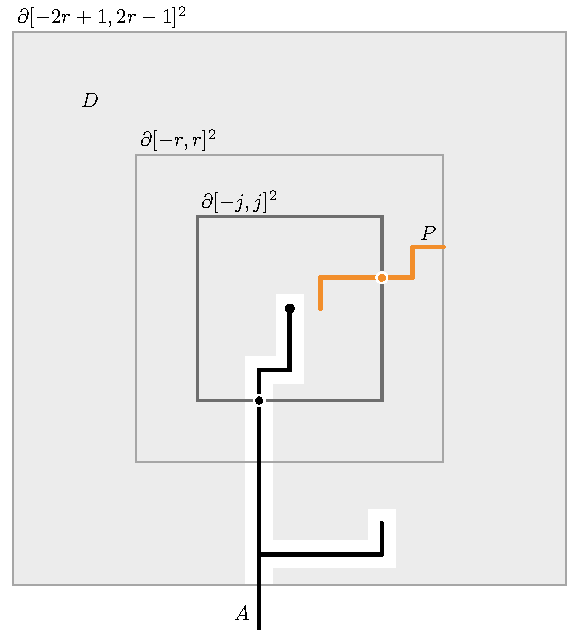
\includegraphics[width=0.6\textwidth]{figures/finite-domain/figure.pdf}
\caption{The domain~$D$, shaded, is the component of~$[-2r+1,2r-1]^2\setminus A$ that contains~$P$, with~$A$ in black and~$P$ in orange. Every square~$\partial[-j,j]^2$ with~$1\leq j\leq r$ meets both~$A$ and~$P$.}
\label{fig:finite-domain}
\end{figure}

\emph{Step 2.} We bound~$\EE Y$ below using the circuits~$\partial[-j,j]^2$. By Proposition~\ref{el:reference-moment}, the mean~$\EE Y$ is the energy of~$\phi$. Extend~$\phi$ to~$\Z^2$ by zero on~$D^c$ and one on~$P$. For~$1\leq j\leq r$, both~$A$ and~$P$ meet the circuit~$\partial[-j,j]^2$, so the circuit has a vertex where~$\phi$ is zero and a vertex where~$\phi$ is one. These two vertices split the circuit into two arcs whose lengths add up to~$8j$. By Cauchy--Schwarz, the edges of each arc contribute at least the reciprocal of the length of the arc to the energy of~$\phi$, so the edges of the circuit contribute at least the sum of these two reciprocals, which is at least~$\nf4{8j}=\nf1{2j}$. The circuits are edge-disjoint and avoid~$e$. Hence
\begin{equation*}
\EE Y\geq\frac12\sum_{j=1}^r\frac1j\geq\frac12\log r\,.
\end{equation*}
Since~$r\geq10^{30}$, this gives~$\EE Y\geq32$ and~$\log r\leq2\,\EE Y$. Since~$D\subset [-2r+1,2r-1]^2$, we also have~$m\leq4|[-2r+1,2r-1]^2|\leq r^3$. Since~$\EE Y\geq1$, the logarithm in~\eqref{el:reference-estimate} is at most~$\log m\leq3\log r$, so~\eqref{el:reference-estimate} gives~$\operatorname{Var}(Y)\leq C\,\EE Y(1+3\log r)\leq4C\,\EE Y\log r\leq8C(\EE Y)^2$, with~$C$ the constant of Proposition~\ref{el:reference-moment}. Hence
\begin{equation*}
\EE[Y^2]=(\EE Y)^2+\operatorname{Var}(Y)\leq(1+8C)(\EE Y)^2\,.
\end{equation*}

\emph{Step 3.} We bound the mean of~$\cL(D^c\setminus A)$ under~$\nu_{D^c,P}$. Since~$D$ is a component of~$[-2r+1,2r-1]^2\setminus A$, every edge from~$D^c\setminus A$ to~$D$ starts outside~$[-2r+1,2r-1]^2$. Every vertex outside~$D$ has color zero, and by~\eqref{fo:color-marginal} a vertex~$y\in D$ has color one with the probability that the walk from~$y$ visits~$P$ before~$D^c$. Since~$P\subset [-r,r]^2$ and~$\Z^2\setminus [-2r+1,2r-1]^2\subset D^c$, this probability is at most the probability that the walk from~$y$ visits~$[-r,r]^2$ before~$\Z^2\setminus [-2r+1,2r-1]^2$. Hence the mean of~$\cL(D^c\setminus A)$ is at most the sum of the latter probability over the edges~$xy$ with~$x\in\Z^2\setminus [-2r+1,2r-1]^2$, which is the effective conductance between~$\Z^2\setminus [-2r+1,2r-1]^2$ and~$[-r,r]^2$ by~\eqref{pre:count-conductance}. Thus~\eqref{pre:annulus} bounds the mean of~$\cL(D^c\setminus A)$ by~$16$.

\emph{Step 4.} We apply the Paley--Zygmund inequality to~$\cL(A)-1$. Since~$e$ joins~$0\in A$ to a vertex of color one, the identity of Step~1 shows that~$\cL(A)-1$ lies between zero and~$Y$ under~$\nu_{D^c,P}$. By Steps~1 and~3, the mean of~$\cL(A)-1$ is at least~$\EE Y-16$, which is at least~$\EE Y/2$ because~$\EE Y\geq32$. By Step~2, the second moment of~$\cL(A)-1$ is at most~$(1+8C)(\EE Y)^2$. Let~$\varepsilon\coloneqq1/(16(1+8C))$, with~$C$ the constant of Proposition~\ref{el:reference-moment}. The Paley--Zygmund inequality gives
\begin{equation*}
\nu_{D^c,P}\bigl(\cL(A)-1\geq\EE Y/4\bigr)\geq\varepsilon\,.
\end{equation*}
Every vertex of color one under~$\nu_{D^c,P}$ lies in~$D\subset [-2r+1,2r-1]^2$, so~$\cL(A)=\cL(A\cap [-2r,2r]^2)$ under~$\nu_{D^c,P}$. The count~$\cL(A\cap [-2r,2r]^2)$ is increasing in the set of vertices of color one, so Step~1 shows that the law of this count under~$\nu_{A,\Gamma}$ stochastically dominates the law under~$\nu_{D^c,P}$. Since~$\EE Y/4\geq\tfrac18\log r$ by Step~2, this proves the proposition.
\end{proof}

\section{Repeating the estimate at many scales}\label{ct:section}

In this section we prove Proposition~\ref{ct:reciprocal} by applying Proposition~\ref{fo:local-comparison} at scales that are fixed powers of their predecessors, as in Step~3 of Section~\ref{ssec:proof-overview}.

\subsection{Roots added inside a box}

In the proof of Proposition~\ref{ct:reciprocal}, the branches of the earlier scales lie in a box~$[-h,h]^2$ with high probability, and we add to the roots of color zero this box joined by a path to a vertex of~$\partial[-2h,2h]^2$, as in Figure~\ref{fig:recentering}. A path along~$\partial[-2h,2h]^2$ could make the effective conductance between the added set and~$\Z^2\setminus [-2h,2h]^2$ proportional to the length of the path. The path in the proof of Lemma~\ref{ct:needle} moves inward at least once in every two steps, and this keeps the effective conductance logarithmic in~$h$.

\begin{figure}[htbp]
\centering
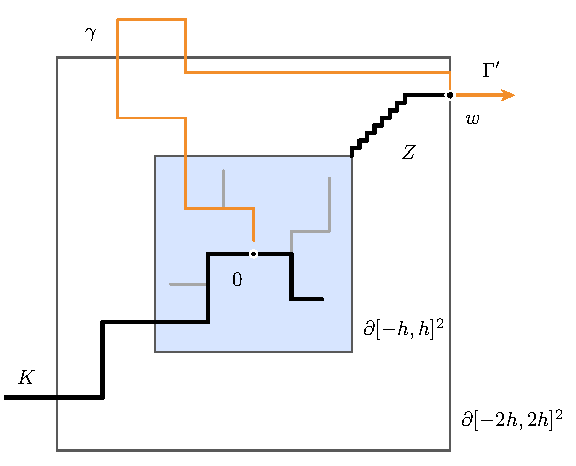
\includegraphics[width=0.55\textwidth]{figures/recentering/figure.pdf}
\caption{The set~$Z$ consists of the shaded box~$[-h,h]^2$, which contains the gray branches of the earlier scales, and the black path from~$[-h,h]^2$ to the vertex~$w$ where~$\gamma$ leaves~$[-2h,2h]^2$ for the last time. Proposition~\ref{fo:local-comparison} applies around~$w$, with the roots~$K\cup Z$ of color zero and~$\Gamma'$ of color one, where~$\Gamma'$, in thick orange, is the component of~$\gamma\setminus [-2h,2h]^2$ with finite complement.}
\label{fig:recentering}
\end{figure}

\begin{lemma}\label{ct:needle}
For every integer~$h\geq10$ and every~$w\in\partial[-2h,2h]^2$, there is a connected set~$Z\subset [-2h,2h]^2$ that contains~$[-h,h]^2$ and~$w$ and for which the effective conductance between~$Z$ and~$\Z^2\setminus [-2h,2h]^2$ is at most~$107\log h$.
\end{lemma}

\begin{proof}
Consider the nearest-neighbor path that starts at~$w$ and, until the path enters~$[-h,h]^2$, steps toward~$0$ in a coordinate of largest absolute value, the first coordinate in case of a tie. Along this path~$|\cdot|_\infty$ never increases and decreases at least once in every two consecutive steps. Let~$Z$ be the union of~$[-h,h]^2$ and the vertices of this path. Then~$Z\subset [-2h,2h]^2$ is connected and contains~$w$.

For each integer~$k\geq1$ with~$2^k<h$, the vertices~$x$ of the path with~$2^k\leq2h-|x|_\infty<2^{k+1}$ are at most~$2^{k+1}$ consecutive vertices of the path. They split into at most four runs of at most~$2^{k-1}$ consecutive vertices. Each run lies in~$x+[-2^{k-1},2^{k-1}]^2$ for its first vertex~$x$, and~$x+[-2^k+1,2^k-1]^2\subset [-2h,2h]^2$ because~$|x|_\infty\leq2h-2^k$. A vertex~$x$ of the path outside~$[-h,h]^2$ with~$|x|_\infty\leq2h-2$ satisfies~$2\leq2h-|x|_\infty<h$ and therefore lies in one of these runs. Hence~$Z$ is the union of~$[-h,h]^2$, of the at most four vertices~$x$ of the path with~$|x|_\infty\geq2h-1$, and of at most~$4\log_2h$ runs.

By~\eqref{pre:count-conductance}, the effective conductance between~$Z$ and~$\Z^2\setminus [-2h,2h]^2$ is the sum, over the edges~$xy$ with~$x\in Z$, of the probability that the walk from~$y$ visits~$\Z^2\setminus [-2h,2h]^2$ before~$Z$. Let~$V$ be one of the sets of this union. Since~$V\subset Z$, the term of each edge~$xy$ with~$x\in V$ is at most the probability that the walk from~$y$ visits~$\Z^2\setminus [-2h,2h]^2$ before~$V$, and by~\eqref{pre:count-conductance} the sum of these bounds over the edges~$xy$ with~$x\in V$ is the effective conductance between~$V$ and~$\Z^2\setminus [-2h,2h]^2$. When~$V$ is a single vertex, this sum has four terms and is at most four. Enlarging either of two sets shrinks the class of functions in~\eqref{pre:dirichlet}, so the effective conductance between the two sets does not decrease, and~\eqref{pre:annulus} and its translates bound the effective conductance between~$V$ and~$\Z^2\setminus [-2h,2h]^2$ by~$16$ when~$V$ is~$[-h,h]^2$ or a run. Summing over~$V$ bounds the effective conductance between~$Z$ and~$\Z^2\setminus [-2h,2h]^2$ by~$32+64\log_2h$, which is at most~$107\log h$ because~$h\geq10$.
\end{proof}

\begin{lemma}\label{ct:revealed-roots}
There is a universal integer~$\kappa\geq30$ such that the following holds, with~$\varepsilon$ as in Proposition~\ref{fo:local-comparison}. Let~$K$ and~$\gamma$ be as in Section~\ref{rd:section}, with~$0\in K$ and with a neighbor of~$0$ in~$\gamma$, and let~$h\geq10$ and~$r\geq h^\kappa$ be integers with~$\diam_\infty K\geq16r$. Let~$A$ and~$\Gamma$ be disjoint sets of vertices with~$K\subset A\subset K\cup [-h,h]^2$ and~$\gamma\subset\Gamma$. Then~$\nu_{A,\Gamma}\bigl(\cL(K\cap [-3r,3r]^2)\geq\tfrac1{16}\log r\bigr)\geq\varepsilon/2$.
\end{lemma}

\begin{proof}
Since~$\gamma$ has finite complement, the set~$\gamma\setminus [-2h,2h]^2$ has a component~$\Gamma'$ with finite complement. Since~$\gamma$ is connected, a simple path in~$\gamma$ joins a neighbor of~$0$ to~$\Gamma'$. Let~$w$ be the last vertex of this path in~$[-2h,2h]^2$. Then~$w\in\partial[-2h,2h]^2$, and~$\Gamma'$ contains the vertices of the path after~$w$, so~$\Gamma'$ contains a neighbor of~$w$. Let~$Z$ be the set given by Lemma~\ref{ct:needle} for~$h$ and~$w$, and let~$A'\coloneqq K\cup Z$, as in Figure~\ref{fig:recentering}. We have~$A\subset K\cup [-h,h]^2\subset A'$ and~$\Gamma'\subset\gamma\subset\Gamma$. Since~$K\cap\gamma=\varnothing$ and~$Z\subset [-2h,2h]^2$, the sets~$A'$ and~$\Gamma'$ are disjoint. The union~$A\cup\Gamma$ contains~$\gamma$ and the union~$A'\cup\Gamma'$ contains~$\Gamma'$, so both unions have finite complements. Lemma~\ref{fo:lattice-monotonicity} therefore shows that the set of vertices of color one is stochastically smaller under~$\nu_{A',\Gamma'}$ than under~$\nu_{A,\Gamma}$.

The set~$A'$ is connected and contains~$w$, and~$A'$ meets~$\Z^2\setminus (w+[-2r+1,2r-1]^2)$, since~$\diam_\infty K\geq16r$. The set~$\Gamma'$ is connected and unbounded and contains a neighbor of~$w$, so~$\Gamma'$ meets~$w+\partial[-r,r]^2$. Since~$r\geq h^\kappa\geq10^{30}$, Proposition~\ref{fo:local-comparison}, translated by~$w$, gives
\begin{equation*}
\nu_{A',\Gamma'}\bigl(\cL(A'\cap (w+[-2r,2r]^2))\geq\tfrac18\log r\bigr)\geq\varepsilon\,.
\end{equation*}

By~\eqref{fo:color-marginal}, the mean of~$\cL(A'\setminus K)$ under~$\nu_{A',\Gamma'}$ is the sum of~$\PP_y(\text{the walk visits~$\Gamma'$ before~$A'$})$ over the edges~$xy$ with~$x\in A'\setminus K$. Since~$A'\setminus K\subset Z\subset A'$ and~$\Gamma'\subset\Z^2\setminus [-2h,2h]^2$, each term is at most~$\PP_y(\text{the walk visits~$\Z^2\setminus [-2h,2h]^2$ before~$Z$})$. By~\eqref{pre:count-conductance}, the sum of these bounds over the edges~$xy$ with~$x\in Z$ is the effective conductance between~$Z$ and~$\Z^2\setminus [-2h,2h]^2$. Lemma~\ref{ct:needle} therefore bounds the mean of~$\cL(A'\setminus K)$ by~$107\log h$.

Choose an integer~$\kappa\geq\max\{30,3424/\varepsilon\}$. Markov's inequality and~$r\geq h^\kappa$ give
\begin{equation*}
\nu_{A',\Gamma'}\bigl(\cL(A'\setminus K)>\tfrac1{16}\log r\bigr)\leq\frac{1712\log h}{\log r}\leq\frac{1712}\kappa\leq\frac\varepsilon2\,.
\end{equation*}
Since~$\cL(A'\cap (w+[-2r,2r]^2))\leq\cL(K\cap (w+[-2r,2r]^2))+\cL(A'\setminus K)$, the count~$\cL(K\cap (w+[-2r,2r]^2))$ is at least~$\tfrac1{16}\log r$ with~$\nu_{A',\Gamma'}$-probability at least~$\varepsilon/2$. Since~$|w|_\infty=2h\leq r$, the box~$w+[-2r,2r]^2$ lies in~$[-3r,3r]^2$. The count~$\cL(K\cap [-3r,3r]^2)$ is increasing in the set of vertices of color one, so the comparison in the first paragraph gives~$\nu_{A,\Gamma}\bigl(\cL(K\cap [-3r,3r]^2)\geq\tfrac1{16}\log r\bigr)\geq\varepsilon/2$.
\end{proof}

\subsection{Exploring the forest scale by scale}

\begin{proof}[Proof of Proposition~\ref{ct:reciprocal}]
Let~$K$ and~$\gamma$ be as in Proposition~\ref{ct:reciprocal}, and translate so that~$0\in K$ and~$\gamma$ contains a neighbor of~$0$.

\emph{Step 1.} We choose the scales. Let~$\kappa$ be as in Lemma~\ref{ct:revealed-roots}. For~$i\geq0$, let~$r_i\coloneqq2^{(6\kappa)^i}$, so that~$r_{i+1}=(r_i^6)^\kappa$. Fix an integer~$n\geq1$ with~$\diam_\infty K\geq16r_{2n-1}$. We use the scales~$r_i$ with~$n-1\leq i\leq2n-1$.

\emph{Step 2.} We explore the forest scale by scale. Run Wilson's algorithm of Section~\ref{ssec:prelim-wilson} with roots~$K$ of color zero and~$\gamma$ of color one, under an enumeration of~$\Z^2$ that lists, for each~$n-1\leq i\leq2n-1$, the vertices of~$[-3r_i-1,3r_i+1]^2$ before the other vertices. The resulting colors have law~$\nu_{K,\gamma}$. For~$n-1\leq i\leq2n-1$, the walks of the scales up to~$i$ are the walks started in~$[-3r_i-1,3r_i+1]^2$. Given the walks of the scales up to~$i$, the later walks use new independent increments and carry out Wilson's algorithm with two root sets: the set~$K$ together with the vertices that the branches of the given walks join to~$K$, and the set~$\gamma$ together with the other vertices of these branches. Hence the conditional law of the colors given these walks is~$\nu_{A,\Gamma}$, where~$A$ and~$\Gamma$ are these two root sets. Every vertex of~$[-3r_i-1,3r_i+1]^2$ is a root after the walks of the scales up to~$i$, and every neighbor of~$K\cap [-3r_i,3r_i]^2$ lies in~$[-3r_i-1,3r_i+1]^2$, so these walks determine~$\cL(K\cap [-3r_i,3r_i]^2)$.

\emph{Step 3.} For~$n-1\leq i\leq2n-2$, we bound the probability that some walk of the scales up to~$i$ leaves~$[-r_i^6,r_i^6]^2$. Since~$r_{2n-1}=(r_{2n-2}^6)^\kappa\geq r_i^6$ and~$0\in K$, some vertex~$x$ of~$K$ satisfies~$|x|_\infty\geq\tfrac12\diam_\infty K\geq r_i^6$, so the connected set~$K$ meets~$\partial[-r_i^6,r_i^6]^2$. Every walk of the scales up to~$i$ starts in~$[-3r_i-1,3r_i+1]^2$ and stops no later than the first visit to~$K$, so such a walk that leaves~$[-r_i^6,r_i^6]^2$ visits~$\partial[-r_i^6,r_i^6]^2$ strictly before~$K$. Given the earlier walks, the bound~\eqref{ct:beurling} for~$K$ with~$r_i$ in place of~$r$ bounds the probability that a given walk of the scales up to~$i$ leaves~$[-r_i^6,r_i^6]^2$ by~$Cr_i^{-\nf52}$. Summing over the at most~$(6r_i+3)^2$ walks of the scales up to~$i$ bounds the probability that some walk of the scales up to~$i$ leaves~$[-r_i^6,r_i^6]^2$ by~$Cr_i^{-\nf12}$.

\emph{Step 4.} Let~$n\leq i\leq2n-1$. We show that, given the walks of the scales up to~$i-1$, on the event that these walks stay in~$[-r_{i-1}^6,r_{i-1}^6]^2$, the conditional probability that~$\cL(K\cap [-3r_i,3r_i]^2)\geq\tfrac1{16}\log r_n$ is at least~$\varepsilon/2$. Let~$A$ and~$\Gamma$ be the root sets after the walks of the scales up to~$i-1$, as in Step~2. Then~$K\subset A$ and~$\gamma\subset\Gamma$, and on this event every branch of these walks lies in~$[-r_{i-1}^6,r_{i-1}^6]^2$, so~$A\subset K\cup [-r_{i-1}^6,r_{i-1}^6]^2$. Since~$r_{i-1}^6\geq64$ and~$r_i=(r_{i-1}^6)^\kappa$, and since~$\diam_\infty K\geq16r_{2n-1}\geq16r_i$, Lemma~\ref{ct:revealed-roots} with~$h=r_{i-1}^6$ and~$r=r_i$ applies to~$\nu_{A,\Gamma}$, which is the conditional law of the colors by Step~2. Since~$r_n\leq r_i$, this proves the claim.

\emph{Step 5.} We multiply the conditional failure bounds. Consider the event that, for every~$n\leq i\leq2n-1$, the walks of the scales up to~$i-1$ stay in~$[-r_{i-1}^6,r_{i-1}^6]^2$ and~$\cL(K\cap [-3r_i,3r_i]^2)<\tfrac1{16}\log r_n$. For each~$n\leq i\leq2n-1$, the walks of the scales up to~$i-1$ determine whether these conditions hold for the indices from~$n$ to~$i-1$ and whether these walks stay in~$[-r_{i-1}^6,r_{i-1}^6]^2$. On the event that these walks stay in~$[-r_{i-1}^6,r_{i-1}^6]^2$, Step~4 bounds the conditional probability that~$\cL(K\cap [-3r_i,3r_i]^2)<\tfrac1{16}\log r_n$ by~$1-\varepsilon/2$. Induction over~$i$ therefore bounds the probability of the event by~$(1-\varepsilon/2)^n$. If~$\cL(K)<\tfrac1{16}\log r_n$, then~$\cL(K\cap [-3r_i,3r_i]^2)<\tfrac1{16}\log r_n$ for every~$i$, so either this event occurs or, for some~$n-1\leq i\leq2n-2$, some walk of the scales up to~$i$ leaves~$[-r_i^6,r_i^6]^2$. Step~3 and~$r_{i+1}\geq r_i^4$ give
\begin{equation*}
\nu_{K,\gamma}\bigl(\cL(K)<\tfrac1{16}\log r_n\bigr)\leq(1-\varepsilon/2)^n+C\sum_{i=n-1}^{2n-2}r_i^{-\nf12}\leq(1-\varepsilon/2)^n+2Cr_{n-1}^{-\nf12}\,.
\end{equation*}

\emph{Step 6.} We deduce the bound of Proposition~\ref{ct:reciprocal}. Since~$\cL(K)\geq1$ and~$\log r_n=(6\kappa)^n\log2$, and since~$(6\kappa)^{-1}<\nf12<1-\varepsilon/2$, we obtain
\begin{equation*}
\begin{split}
\EE_{\nu_{K,\gamma}}\bigl[\cL(K)^{-1}\bigr]&\leq\nu_{K,\gamma}\bigl(\cL(K)<\tfrac1{16}\log r_n\bigr)+\frac{16}{\log r_n}\\
&\leq(1-\varepsilon/2)^n+2Cr_{n-1}^{-\nf12}+\frac{16}{(6\kappa)^n\log2}\leq C(1-\varepsilon/2)^n\,.
\end{split}
\end{equation*}
For~$\diam_\infty K\geq16r_1$, apply this bound with the largest~$n$ such that~$16r_{2n-1}\leq\diam_\infty K$. Then~$\diam_\infty K<16r_{2n+1}$, so~$\log(\diam_\infty K+2)\leq\log18+(6\kappa)^{2n+1}\log2\leq C(6\kappa)^{2n}$. Let~$a\coloneqq-\log(1-\varepsilon/2)/(2\log(6\kappa))$, which is positive. The previous display then gives
\begin{equation*}
\EE_{\nu_{K,\gamma}}\bigl[\cL(K)^{-1}\bigr]\leq C(1-\varepsilon/2)^n=C(6\kappa)^{-2an}\leq C\bigl(\log(\diam_\infty K+2)\bigr)^{-a}\,.
\end{equation*}
Since~$\cL(K)\geq1$, increasing~$C$ extends the bound to~$\diam_\infty K<16r_1$.
\end{proof}

\section{A second moment for boundary edges}\label{sec:electrical}

In this section we prove Proposition~\ref{el:reference-moment}. By planar duality, $Y$ is the number of edges that a path on the boundary of a dual graph shares with the path between the endpoints of this boundary path in a uniform spanning tree of the dual graph. Identities of~\citet*{KenyonWilson2009} express the probability that this tree path contains two given edges of the boundary path through the Green function of the dual graph, and summing over pairs of edges reduces the variance bound to bounds on this Green function along the boundary path. We prove these bounds with test functions built in the coordinates of the electrical square tiling.

\subsection{Edges on a boundary path}\label{ssec:boundary-path}

Adding~$e$ to the uniform rooted spanning forest of~$H_0$ defined before Proposition~\ref{el:reference-moment} gives a uniform spanning tree of~$H$ conditioned to contain~$e$. Let the dual graph be the graph obtained from the plane dual of~$H$ by deleting the edge dual to~$e$. The duals of the edges absent from the tree form a uniform spanning tree of the dual graph~\citep[Proposition~12.1]{BLPS2001}. The edges incident to~$\alpha$ form a minimal cut of~$H$, because~$H\setminus\{\alpha\}$ is connected. Their duals therefore form a simple cycle through the edge dual to~$e$, and deleting that edge leaves a simple path~$v_0,\ldots,v_m$ in the dual graph. The~$m$ edges of this path are the duals of the edges of~$H_0$ incident to~$\alpha$. Deleting the edge dual to~$e$ also merges the faces of the plane dual that correspond to~$\alpha$ and~$\beta$, and we take the merged face as the outer face of the dual graph. The path~$v_0,\ldots,v_m$ lies on the boundary of this face, since the cycle bounds the face corresponding to~$\alpha$. The dual graph lies in the closed disk that the cycle bounds on the other side, and we take the cyclic order around the outer face to be the order along this cycle, in the direction in which~$v_0,\ldots,v_m$ occur in this order.

For~$0\leq i<m$, let~$e_i$ be the edge of~$H_0$ whose dual is the edge of the path~$v_0,\ldots,v_m$ from~$v_i$ to~$v_{i+1}$, and let~$I_i$ be the indicator that the dual of~$e_i$ lies on the path from~$v_0$ to~$v_m$ in the uniform spanning tree of the dual graph. An edge~$\alpha x$ of~$H_0$ joins the two components of the forest exactly when adding~$\alpha x$ to the tree of~$H$ creates a cycle through~$e$. By planar cycle-cut duality, this holds exactly when the dual of~$\alpha x$ lies on the path from~$v_0$ to~$v_m$ in the spanning tree of the dual graph, as in Figure~\ref{fig:dual-path}. Hence~$I_i$ is the indicator that the endpoint other than~$\alpha$ of~$e_i$ has color one, and~$Y=\sum_iI_i$.

\begin{figure}[htbp]
\centering
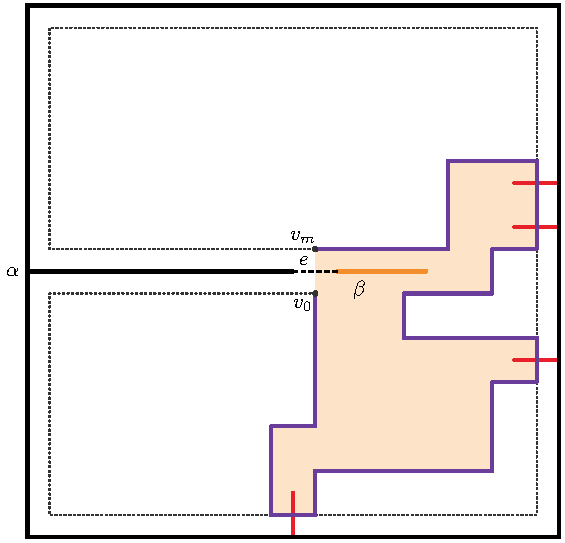
\includegraphics[width=0.6\textwidth]{figures/dual-path/figure.pdf}
\caption{The duals of the edges at~$\alpha$ form the dotted path~$v_0,\ldots,v_m$, and the purple path from~$v_0$ to~$v_m$ in the spanning tree of the dual graph, together with the dual of~$e$, bounds the shaded set of vertices of color one. Hence the purple path runs along the dotted path exactly across the red edges, which join~$\alpha$ to vertices of color one.}
\label{fig:dual-path}
\end{figure}

Let~$\mathcal G$ be the Green function of the dual graph grounded at~$v_m$, so that~$\mathcal G(x,y)$ is the voltage at~$y$ when unit current enters the dual graph at~$x$ and leaves at~$v_m$, and the voltage at~$v_m$ is zero. For~$0\leq i\leq m$, let~$\psi_i\coloneqq\mathcal G(v_0,v_i)$ and~$g_i\coloneqq\mathcal G(v_i,v_i)$, and for~$0\leq i<m$, let~$p_i\coloneqq\psi_i-\psi_{i+1}$, which is the current through the dual of~$e_i$ when unit current flows from~$v_0$ to~$v_m$. Then~$\psi_m=g_m=0$ and~$g_0=\psi_0$.

A simple path from~$v_0$ to~$v_m$ in the dual graph uses the dual of each~$e_i$ only from~$v_i$ to~$v_{i+1}$, and uses these duals in increasing order of~$i$. Indeed, two disjoint paths cannot join two pairs of vertices on the boundary of the outer face that alternate in the cyclic order around that face~\citep[Section~1.1]{KenyonWilson2011}. A backward traversal of the dual of~$e_i$ would either repeat~$v_0$ or~$v_m$, or give disjoint initial and final segments from~$v_0$ to~$v_{i+1}$ and from~$v_i$ to~$v_m$, whose endpoints alternate. If the path uses the dual of~$e_j$ before the dual of~$e_i$, where~$i<j$, the path repeats~$v_{i+1}$ when~$j=i+1$. Otherwise the initial segment to~$v_j$ and the final segment from~$v_{i+1}$ are disjoint and again have alternating endpoints.

By Kirchhoff's theorem~\citep[Exercise~4.23]{LyonsPeres2016}, the current~$p_i$ is the probability that the tree path from~$v_0$ to~$v_m$ traverses the dual of~$e_i$ from~$v_i$ to~$v_{i+1}$ minus the probability that this path traverses this dual edge from~$v_{i+1}$ to~$v_i$. The second probability is zero, so~$p_i=\EE I_i$. Let~$x$ be the endpoint other than~$\alpha$ of~$e_i$. By~\eqref{pre:wilson} with~$x$ enumerated first and by~\eqref{pre:voltage}, the vertex~$x$ has color one with probability~$\phi(x)$. Hence~$p_i=\phi(x)$, which is the current through~$e_i$ and is positive because~$D$ is connected and contains~$P$. Therefore~$\psi_0=\sum_ip_i$ is the sum of~$\phi(x)$ over the edges~$\alpha x$ of~$H_0$, which is the energy of~$\phi$ by~\eqref{pre:voltage} and~\eqref{pre:count-conductance}. Hence
\begin{equation*}
 \EE Y=\sum_{i=0}^{m-1}p_i=\psi_0\,.
\end{equation*}

\begin{lemma}\label{el:pair-contact}
For every~$0\leq i<j<m$ we have
\begin{align}\label{el:pair-expanded}
 \EE[I_iI_j]
 &=\psi_i\bigl(\mathcal G(v_{i+1},v_j)-\mathcal G(v_{i+1},v_{j+1})\bigr)
   -\psi_{i+1}\bigl(\mathcal G(v_i,v_j)-\mathcal G(v_i,v_{j+1})\bigr)\notag\\
 &\quad-\psi_j\bigl(\mathcal G(v_i,v_{j+1})-\mathcal G(v_{i+1},v_{j+1})\bigr)
   +\psi_{j+1}\bigl(\mathcal G(v_i,v_j)-\mathcal G(v_{i+1},v_j)\bigr)\,.
\end{align}
\end{lemma}

\begin{proof}
Assume first that the six vertices of the tuple~$(v_m,v_0,v_i,v_{i+1},v_j,v_{j+1})$ are distinct. Number them from~1 to~6 in this order, which is their cyclic order around the outer face, and call them the nodes. We write a partition of the nodes into pairs by the numbers in its pairs, for example~$16|23|45$. A simple path from~$v_0$ to~$v_m$ that uses the duals of~$e_i$ and~$e_j$ traverses the dual of~$e_i$ from~$v_i$ to~$v_{i+1}$ and then the dual of~$e_j$ from~$v_j$ to~$v_{j+1}$. Hence deleting these two dual edges from a spanning tree of the dual graph whose path from~$v_0$ to~$v_m$ uses both dual edges leaves a spanning forest with three components that contain the pairs of~$16|23|45$, one pair each. Conversely, adding these two dual edges to such a forest gives a spanning tree whose path from~$v_0$ to~$v_m$ uses both dual edges. Thus~$\EE[I_iI_j]$ is the number of these forests divided by the number of spanning trees of the dual graph.

Consider two disjoint triples of nodes, the first containing node~1 and the second containing node~6, and list each triple in increasing order. By~\citet*[Theorems~8.1 and~B.3]{KenyonWilson2009}, two quantities agree. The first is a sum over the six partitions of the nodes into pairs that each contain one node of each triple. Each such partition contributes the sign of the permutation that its pairs induce between the two lists, times the number of spanning forests with three components that contain its pairs, one pair each, divided by the number of spanning trees. The second is the coefficient of the linear term of the polynomial in one variable obtained as the determinant of the three-by-three matrix whose rows correspond to the first triple, whose columns correspond to the second triple, and whose entry for nodes~$x$ and~$y$ is this variable minus half the effective resistance~$\mathcal G(x,x)+\mathcal G(y,y)-2\mathcal G(x,y)$ between~$x$ and~$y$. Since node~1 is~$v_m$ and~$\mathcal G(v_m,\cdot)=0$, subtracting the row of node~1 from the other two rows and then the column of node~6 from the other two columns leaves the variable only in the entry for nodes~1 and~6. The cofactor of this entry has positive sign and is the determinant of the two-by-two matrix with entries~$\mathcal G(x,y)-\mathcal G(x,v_{j+1})$ for~$x$ in the first triple other than node~1 and~$y$ in the second triple other than node~6.

By planarity, the partition of the nodes induced by a spanning forest is noncrossing~\citep[Section~1.1]{KenyonWilson2011}: no two of its pairs alternate around the outer face. For the triples~$124$ and~$356$, the only noncrossing partitions in the sum are~$16|23|45$, with sign~$+1$, and~$16|25|34$, with sign~$-1$. For the triples~$123$ and~$456$, only~$16|25|34$ occurs, with sign~$-1$. Subtracting the second identity from the first cancels the partition~$16|25|34$. Since node~2 is~$v_0$, the entries in the row of node~2 are differences of the numbers~$\psi_0,\ldots,\psi_m$, and
\begin{align*}
\EE[I_iI_j]
&=\det\begin{pmatrix}
\psi_i-\psi_{j+1}&\psi_j-\psi_{j+1}\\
\mathcal G(v_{i+1},v_i)-\mathcal G(v_{i+1},v_{j+1})&\mathcal G(v_{i+1},v_j)-\mathcal G(v_{i+1},v_{j+1})
\end{pmatrix}\\
&\quad-\det\begin{pmatrix}
\psi_{i+1}-\psi_{j+1}&\psi_j-\psi_{j+1}\\
\mathcal G(v_i,v_{i+1})-\mathcal G(v_i,v_{j+1})&\mathcal G(v_i,v_j)-\mathcal G(v_i,v_{j+1})
\end{pmatrix}\,.
\end{align*}
Expanding the two determinants and using the symmetry of~$\mathcal G$ gives~\eqref{el:pair-expanded}.

Only three coincidences among the six vertices can occur: nodes~2 and~3 coincide when~$i=0$, nodes~4 and~5 when~$j=i+1$, and nodes~6 and~1 when~$j=m-1$. For each coincidence, attach a new vertex by a pendant edge to the vertex that serves as both nodes, and use the new vertex as node~3 or~5 or~6, respectively. We draw each pendant edge outside the closed disk that contains the dual graph, so that the enlarged graph lies in a closed disk with the six nodes on its boundary in the order of their numbers, and we take this order as their cyclic order around the outer face. Each pendant edge lies in every spanning tree and in every forest counted above, since otherwise its new vertex would form a component with one node, so no count changes. The Green function of the enlarged graph, grounded at~$v_m$, extends~$\mathcal G$ and takes at each new vertex the values of~$\mathcal G$ at the only neighbor of the new vertex, except on the diagonal, which neither determinant uses. Hence~\eqref{el:pair-expanded} holds in all cases.
\end{proof}

\begin{lemma}\label{el:arc-moment}
We have
\begin{equation*}
 \operatorname{Var}(Y)\leq\EE Y+3\sum_{i=0}^{m-1}p_i\bigl(g_i-\psi_i+g_{i+1}-\psi_{i+1}\bigr)\,.
\end{equation*}
\end{lemma}

\begin{proof}
Sum the first two terms of~\eqref{el:pair-expanded} over~$j$ and the last two over~$i$. Since~$\mathcal G(\cdot,v_m)=0$, the Green-function differences telescope, and adding the vanishing terms~$\psi_{m-1}g_m-\psi_m\mathcal G(v_{m-1},v_m)$ and~$\psi_0\mathcal G(v_0,v_1)-\psi_1g_0=\psi_0\psi_1-\psi_1\psi_0$ gives the first equality in
\begin{equation*}
 \sum_{i<j}\EE[I_iI_j]
 =\sum_{i=0}^{m-1}\bigl(\psi_ig_{i+1}-\psi_{i+1}g_i+p_i\mathcal G(v_i,v_{i+1})\bigr)
 =\sum_{i=0}^{m-1}p_i\bigl(g_i-\psi_i+g_{i+1}-\psi_{i+1}+\mathcal G(v_i,v_{i+1})\bigr)\,.
\end{equation*}
The second equality follows by summation by parts from~$\psi_ig_{i+1}-\psi_{i+1}g_i=\psi_i(g_{i+1}-\psi_{i+1})-\psi_{i+1}(g_i-\psi_i)$, since~$g_0-\psi_0=g_m-\psi_m=0$. Since~$\mathcal G$ is positive semidefinite, we have~$2\mathcal G(v_i,v_{i+1})\leq g_i+g_{i+1}$. Multiplying by~$p_i>0$ and using~$\sum_ip_i(\psi_i+\psi_{i+1})=\sum_i(\psi_i^2-\psi_{i+1}^2)=\psi_0^2$ bounds the pair sum by~$\tfrac12\psi_0^2+\tfrac32\sum_ip_i(g_i-\psi_i+g_{i+1}-\psi_{i+1})$. Since~$I_i^2=I_i$ and~$\EE Y=\psi_0$, doubling the pair sum, adding~$\sum_i\EE I_i=\EE Y$, and subtracting~$(\EE Y)^2$ proves the lemma.
\end{proof}

\subsection{Electrical coordinates}

To bound~$g_i-\psi_i$, we use the voltage and stream-function coordinates of the electrical square tiling of~\citet*{BrooksSmithStoneTutte1940}; see also~\citet[Section~9.6]{LyonsPeres2016}.

Since~$H_0$ is connected, the edge~$e$ is not a bridge of~$H$, and deleting~$e$ merges the two faces of~$H$ on either side of~$e$, which correspond to~$v_0$ and~$v_m$, into one face of~$H_0$ whose boundary contains~$\alpha$ and~$\beta$. We take this face as the outer face of~$H_0$. Every vertex of~$D\setminus P$ has degree four in~$H_0$, and~$\phi$ is harmonic there. The edges~$e_0,\ldots,e_{m-1}$ appear around~$\alpha$ in this order, from one side of the outer face to the other.

Draw an auxiliary arc from~$\alpha$ to~$\beta$ that divides the outer face into two. By Kirchhoff's current law, there is a stream function on the resulting faces, unique up to an additive constant, whose increment from the face on the right of each edge, relative to the direction of the current, to the face on the left is the current through that edge. Use the voltage as the horizontal coordinate and the stream function as the vertical coordinate. For an edge~$xy$ with positive current~$|\phi(x)-\phi(y)|$, the \textbf{square} of~$xy$ is the product of the interval between~$\phi(x)$ and~$\phi(y)$ and the interval between the stream values of the two faces on either side of~$xy$. Both intervals have length~$|\phi(x)-\phi(y)|$. An edge of zero current defines a point, at the common voltage of its endpoints and the common stream value of the two faces on either side. Figure~\ref{fig:electrical-tiling} shows both cases. By the proof of~\citet*[Theorem~(4.31)]{BrooksSmithStoneTutte1940}, the squares have disjoint interiors.

\begin{figure}[htbp]
\centering
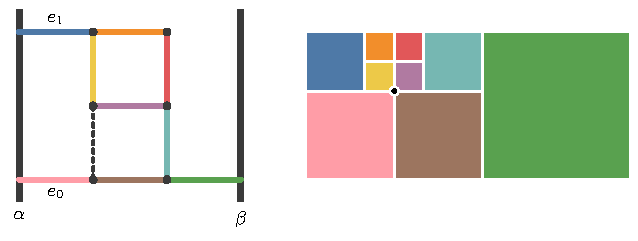
\includegraphics[width=0.85\textwidth]{figures/electrical-tiling/electrical-tiling.pdf}
\caption{Each edge of the network on the left, whose sides~$\alpha$ and~$\beta$ have voltages zero and one, corresponds to the square of the same color on the right, whose side is the current through the edge. The squares of the edges~$e_0$ and~$e_1$ at~$\alpha$ lie along the left side of the rectangle in the order of these edges around~$\alpha$. The dashed edge has zero current, and its square degenerates to the black point.}
\label{fig:electrical-tiling}
\end{figure}

For~$0<i<m$, split~$\alpha$ into a vertex~$\alpha_0$ that receives~$e_0,\ldots,e_{i-1}$ and a vertex~$\alpha_1$ that receives~$e_i,\ldots,e_{m-1}$. Extend~$\phi$ to the split network by zero at~$\alpha_0$ and at~$\alpha_1$.

\begin{lemma}\label{el:split-estimate}
For every~$0<i<m$ and~$j\in\{i-1,i\}$ we have
\begin{equation*}
 g_i-\psi_i\leq1+3888\Bigl(1+\log\frac2{p_j}\Bigr)\,.
\end{equation*}
\end{lemma}

\begin{proof}
\emph{Step 1.} We reduce the bound to a weighted energy. Add to the dual graph an edge from~$v_i$ to~$v_m$ that bounds a face together with the path~$v_i,\ldots,v_m$. The plane dual of the resulting graph is the split network with~$\alpha_0$ and~$\beta$ identified, together with the dual of the added edge, which joins~$\alpha_1$ to the identified vertex. Both the dual graph and the split network with~$\alpha_0$ and~$\beta$ identified are connected, so by~\citet[Proposition~9.4]{LyonsPeres2016}, the effective resistance~$g_i$ between~$v_i$ and~$v_m$ in the dual graph equals the effective conductance between~$\alpha_1$ and~$\{\alpha_0,\beta\}$ in the split network.

Let~$f$ be a function on the vertices of the split network with~$f(\alpha_0)=0$ and~$f(\alpha_1)=1$. Every edge~$xy$ satisfies
\begin{multline*}
 \bigl((1-\phi(x))f(x)-(1-\phi(y))f(y)\bigr)^2=(1-\phi(x))(1-\phi(y))(f(x)-f(y))^2\\
 +(\phi(y)-\phi(x))\bigl((1-\phi(x))f(x)^2-(1-\phi(y))f(y)^2\bigr)\,.
\end{multline*}
Summed over the edges, the last terms give the sum over the vertices~$x$ of~$(1-\phi(x))f(x)^2$ times the net current into~$x$, which is the sum of~$\phi(y)-\phi(x)$ over the edges~$xy$ at~$x$. The net current vanishes at every vertex of~$D\setminus P$, the factor~$1-\phi$ vanishes at~$\beta$, and~$f$ vanishes at~$\alpha_0$. At~$\alpha_1$, the term is the sum of~$\phi(y)$ over the edges~$\alpha_1y$, which is~$p_i+\cdots+p_{m-1}=\psi_i$. Hence the energy of~$(1-\phi)f$ is~$\psi_i$ plus the sum over the edges of the first term on the right side of the previous display. The function~$(1-\phi)f$ is zero at~$\alpha_0$ and at~$\beta$ and one at~$\alpha_1$, so~\eqref{pre:dirichlet} bounds~$g_i$ by this energy, and
\begin{equation*}
 g_i-\psi_i\leq\sum_{xy}(1-\phi(x))(1-\phi(y))(f(x)-f(y))^2\,,
\end{equation*}
where the sum runs over the edges of the split network.

\emph{Step 2.} We choose coordinates and a function on the plane. Between consecutive faces around~$\alpha$, the stream value changes by the current through the edge that separates these faces, always in the same direction, since every such current flows into~$\alpha$. Hence the squares of the edges at~$\alpha$ have their left sides on the vertical axis and follow one another along the axis in the order of these edges around~$\alpha$, so the squares of the edges at~$\alpha_0$ lie on one side of those of the edges at~$\alpha_1$. Reflect the vertical coordinate if necessary so that the squares of the edges at~$\alpha_0$ lie below. Choose the additive constant of the stream function so that the center of the square of~$e_j$ has vertical coordinate zero, and multiply both coordinates by~$2/p_j$. Then the squares have disjoint interiors and lie in the strip of points whose horizontal coordinate lies between zero and~$2/p_j$. The square of~$e_j$ has side two, the squares of the other edges at~$\alpha_0$ lie below height~$-1$, and those of the other edges at~$\alpha_1$ lie above height~$1$. For a point~$z$ of the plane with vertical coordinate~$z_2$, let
\begin{equation*}
 F(z)\coloneqq\frac12+\frac{z_2}{2\max\{1,|z|_\infty\}}\,.
\end{equation*}
Then~$0\leq F\leq1$, and on the vertical axis~$F$ equals zero below height~$-1$ and one above height~$1$. Figure~\ref{fig:split-coordinates} shows these coordinates and the level lines of~$F$. For an axis-parallel square~$Q$, let~$\operatorname{osc}_QF\coloneqq\max_QF-\min_QF$. Since~$|z_2|\leq\max\{1,|z|_\infty\}$ and the functions~$z\mapsto z_2$ and~$z\mapsto\max\{1,|z|_\infty\}$ are~$1$-Lipschitz for~$|\cdot|_\infty$, every such square~$Q$ satisfies
\begin{equation}\label{el:max-angular-osc}
 \operatorname{osc}_QF\leq\frac{\diam_\infty Q}{\max\{1,\min_Q|\cdot|_\infty\}}\,.
\end{equation}

\begin{figure}[htbp]
\centering
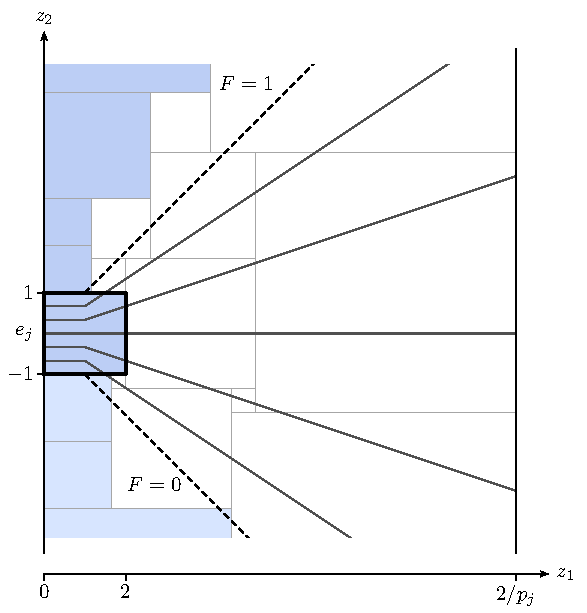
\includegraphics[width=0.6\textwidth]{figures/split-coordinates/figure.pdf}
\caption{In the coordinates of Step~2 of the proof of Lemma~\ref{el:split-estimate}, the square of~$e_j$ is~$[0,2]\times[-1,1]$, the squares of the other edges at~$\alpha_0$ and~$\alpha_1$ lie below and above this square on the vertical axis, and the gray level lines of~$F$ are rays from the origin outside the unit box.}
\label{fig:split-coordinates}
\end{figure}

\emph{Step 3.} We choose the values of~$f$ and compare them with~$F$. Let~$f$ be zero at~$\beta$. Let~$x\in D\setminus P$, and let the segment of~$x$ be the vertical segment at the horizontal coordinate of~$x$ that joins the smallest and the largest stream values of the faces at~$x$. Between consecutive faces around~$x$, the stream value changes by the current through the edge that separates these faces, and these changes add up to zero because~$\phi$ is harmonic at~$x$. Hence the segment of~$x$ has length at most half the sum of the absolute values of the four changes, and so at most twice the largest of them. This segment contains the side at that coordinate of the square of every edge at~$x$, and the point of every edge at~$x$ of zero current. Let~$f(x)$ be the value of~$F$ at the midpoint of the segment. If some edge at~$x$ has positive current, let~$Q_x$ be a largest square of an edge at~$x$. The segment contains a side of~$Q_x$ and has length at most twice the side of~$Q_x$, so the concentric dilation~$3Q_x$ contains the segment, and~$f(x)$ differs from the value of~$F$ at every point of the segment by at most~$\operatorname{osc}_{3Q_x}F$. Otherwise the segment is a point, and~$f(x)$ is the value of~$F$ there.

Let~$xy$ be an edge of the split network that is not incident to~$\beta$ and is not~$e_j$. If~$xy$ has positive current, compare~$f(x)$ and~$f(y)$ through the midpoints of the two vertical sides of the square~$Q$ of~$xy$. The values of~$F$ at these midpoints differ by at most~$\operatorname{osc}_QF\leq\operatorname{osc}_{3Q}F$. At an endpoint in~$D\setminus P$, the midpoint lies in the segment of the endpoint. At an endpoint~$\alpha_0$ or~$\alpha_1$, the midpoint lies on the vertical axis below height~$-1$ or above height~$1$, so the value of~$F$ there equals the value of~$f$ at that endpoint. If~$xy$ has zero current, both endpoints lie in~$D\setminus P$, since the edges at~$\alpha_0$ and~$\alpha_1$ have positive currents, and we compare~$f(x)$ and~$f(y)$ with the value of~$F$ at the point of~$xy$, which lies in the segments of~$x$ and~$y$. In both cases~$|f(x)-f(y)|$ is at most the sum of~$\operatorname{osc}_{3Q}F$ if~$xy$ has positive current, of~$\operatorname{osc}_{3Q_x}F$ if~$x$ lies in~$D\setminus P$ and has an edge of positive current, and of~$\operatorname{osc}_{3Q_y}F$ under the same condition on~$y$. The square of a sum of three numbers is at most three times the sum of their squares. The square of an edge equals~$Q_x$ only if~$x$ is an endpoint of this edge, and each~$Q_x$ enters the bounds for at most the four edges at~$x$. The weight~$(1-\phi(x))(1-\phi(y))$ is at most one and vanishes on the edges at~$\beta$, and the term of~$e_j$ in the following sum is at most one, since~$0\leq f\leq1$. Hence
\begin{equation*}
 \sum_{xy}(1-\phi(x))(1-\phi(y))(f(x)-f(y))^2\leq1+27\sum_Q\bigl(\operatorname{osc}_{3Q}F\bigr)^2\,,
\end{equation*}
where~$Q$ ranges over the squares of the edges.

\emph{Step 4.} We sum the oscillations. Let~$Q$ be the square of an edge, and let~$z\in Q$. Every point of~$3Q$ lies within~$|\cdot|_\infty$-distance~$2\diam_\infty Q$ of~$z$. If~$|z|_\infty\geq4\diam_\infty Q$, then~$\min_{3Q}|\cdot|_\infty\geq|z|_\infty/2$, and~\eqref{el:max-angular-osc} for~$3Q$ gives
\begin{equation}\label{el:square-osc}
 \operatorname{osc}_{3Q}F\leq\frac{6\diam_\infty Q}{\max\{1,|z|_\infty\}}\,.
\end{equation}
If~$|z|_\infty<4\diam_\infty Q$, then~\eqref{el:square-osc} follows from the bound~$\operatorname{osc}_{3Q}F\leq3\diam_\infty Q$ given by~\eqref{el:max-angular-osc} when~$4\diam_\infty Q\leq1$, and from~$\operatorname{osc}_{3Q}F\leq1$ otherwise. Squaring~\eqref{el:square-osc} and averaging over~$z\in Q$ bounds~$(\operatorname{osc}_{3Q}F)^2$ by~$36$ times the integral of~$\max\{1,|z|_\infty\}^{-2}$ over~$Q$. Along each vertical line, the integral of~$\max\{1,|z|_\infty\}^{-2}$ is four divided by the larger of one and the horizontal coordinate of the line. Integrating this quantity over the horizontal coordinates from zero to~$2/p_j$, which is at least two because every current is at most one, gives~$4\bigl(1+\log(2/p_j)\bigr)$. Since the squares have disjoint interiors and lie in the strip of Step~2, we obtain
\begin{equation*}
 \sum_Q\bigl(\operatorname{osc}_{3Q}F\bigr)^2\leq144\Bigl(1+\log\frac2{p_j}\Bigr)\,.
\end{equation*}
Combining this bound with Steps~1 and~3 and using~$27\cdot144=3888$ proves the lemma.
\end{proof}

\subsection{\texorpdfstring{Proof of Proposition~\ref{el:reference-moment}}{Proof of the variance bound}}

\begin{proof}
Section~\ref{ssec:boundary-path} shows that~$\EE Y$ is the energy of~$\phi$ and that~$g_0-\psi_0=g_m-\psi_m=0$. Let~$0\leq i<m$. When~$i>0$, Lemma~\ref{el:split-estimate} with~$j=i$ bounds~$g_i-\psi_i$ by~$1+3888(1+\log(2/p_i))$. When~$i+1<m$, the same lemma with~$i+1$ in place of~$i$ and with~$j=i$ gives the same bound for~$g_{i+1}-\psi_{i+1}$. Hence
\begin{equation*}
 g_i-\psi_i+g_{i+1}-\psi_{i+1}\leq2+7776\Bigl(1+\log\frac2{p_i}\Bigr)\,.
\end{equation*}
Jensen's inequality for the concave logarithm with weights~$p_i/\EE Y$ gives~$\sum_ip_i\log(1/p_i)\leq\EE Y\log(m/\EE Y)$. Multiplying the previous display by~$p_i$, summing over~$i$, and applying Lemma~\ref{el:arc-moment} gives
\begin{equation*}
 \operatorname{Var}(Y)\leq\EE Y+6\,\EE Y+23328\,\EE Y\Bigl(1+\log2+\log\frac m{\EE Y}\Bigr)\,.
\end{equation*}
Every~$p_i$ is at most one, so~$\EE Y\leq m$ and~$\log(m/\EE Y)\geq0$. Since~$7+23328(1+\log2)\leq4\cdot10^4$, this proves Proposition~\ref{el:reference-moment} with~$C=4\cdot10^4$.
\end{proof}

\bibliographystyle{plainnat}
\bibliography{references}
\end{document}
